\documentclass[aspectratio=169,11pt]{beamer}

% Shared style (ib-tutorials.sty at the repo root).
\makeatletter\def\input@path{{./}{../}}\makeatother
\usepackage{ib-tutorials}

\usepackage[utf8]{inputenc}
\usepackage{amsmath,amssymb}
\usepackage{booktabs}
\usepackage{array}
\newcolumntype{L}[1]{>{\raggedright\arraybackslash}p{#1}}
\usepackage{graphicx}
\graphicspath{{../pictures/4-ibfe/}{pictures/4-ibfe/}}
\usepackage{xcolor}
\usepackage{listings}
\usepackage{tikz}
\usetikzlibrary{arrows.meta,positioning,shapes.geometric,fit,calc,decorations.pathmorphing}
\usepackage{hyperref}

\newcommand{\sourcecredit}[1]{\vfill\begin{flushright}\tiny\textcolor{DarkGray}{#1}\end{flushright}}

\lstset{
  basicstyle=\ttfamily\scriptsize\color{BlackGray},
  keywordstyle=\color{NavyBlue}\bfseries,
  commentstyle=\color{DarkGray}\itshape,
  stringstyle=\color{OliveGreen},
  showstringspaces=false,
  columns=fullflexible,
  keepspaces=true,
  breaklines=true,
  breakindent=1em,
  frame=single,
  framerule=0.4pt,
  rulecolor=\color{LightGray},
  backgroundcolor=\color{LightGray!30},
  xleftmargin=0.25em,
  xrightmargin=0.25em
}
\lstdefinestyle{shell}{morecomment=[l]{\#}}
\lstdefinestyle{input}{morecomment=[l]{//}}
\lstdefinestyle{matlab}{morecomment=[l]{\%}}
\lstdefinestyle{python}{morecomment=[l]{\#}}
\lstdefinestyle{data}{}
\lstdefinestyle{tiny}{basicstyle=\ttfamily\tiny\color{BlackGray}}
\lstdefinestyle{inputtiny}{morecomment=[l]{//},basicstyle=\ttfamily\tiny\color{BlackGray}}
\lstdefinestyle{matlabtiny}{morecomment=[l]{\%},basicstyle=\ttfamily\tiny\color{BlackGray}}
\lstdefinestyle{pythontiny}{morecomment=[l]{\#},basicstyle=\ttfamily\tiny\color{BlackGray}}
\lstdefinestyle{cpp}{language=C++,morecomment=[l]{//}}
\lstdefinestyle{cpptiny}{language=C++,morecomment=[l]{//},basicstyle=\ttfamily\tiny\color{BlackGray}}
\lstdefinestyle{cmake}{morecomment=[l]{\#}}

\title[Getting started with IBFE]{Getting started with IBFE}
\subtitle{A finite element structure in IBAMR: the mesh, the stress and force functions, the input keys, the first example run three ways, and the ExodusII output in VisIt}
\author[Miller]{Laura A. Miller}
\institute[UArizona]{Department of Mathematics, University of Arizona}
\date{Using IB Software \textbullet\ Part IV \textbullet\ Chapter 17}

\begin{document}

% 1
\begin{frame}[plain]
\maketutorialtitlepanel{%
\begin{tikzpicture}[scale=0.84]
  % the plate as a strip of triangles
  \foreach \i in {0,...,9} {
    \draw[BlackGray,thin] (0.6+0.3*\i,1.3) -- (0.9+0.3*\i,1.3) -- (0.75+0.3*\i,1.45) -- cycle;
    \draw[BlackGray,thin] (0.75+0.3*\i,1.45) -- (1.05+0.3*\i,1.45) -- (0.9+0.3*\i,1.3) -- cycle;
  }
  \draw[BlackGray,thick] (0.6,1.3) rectangle (3.6,1.45);
  % vorticity blobs at the ends
  \fill[RubineRed!35] (0.45,1.05) ellipse (0.22 and 0.3);
  \fill[NavyBlue!35] (3.75,1.05) ellipse (0.22 and 0.3);
  % the tether arrows
  \draw[-{Stealth[length=2mm]},RubineRed,very thick] (2.1,1.55) -- (2.1,2.25);
  \node[font=\tiny,text=RubineRed] at (2.75,2.05) {$\mathbf{F} = \kappa_s(\mathbf{s}_{\mathrm{target}} - \mathbf{X})$};
  \node[font=\tiny,text=OliveGreen] at (2.1,0.55) {$\mathbb{P} = \mu\,\mathbb{F} - \mu\,\mathbb{F}^{-T}$};
  \node[font=\tiny,text=DarkGray] at (2.1,0.2) {\code{output.ex2}: \code{dX\_0}, \code{dX\_1}};
\end{tikzpicture}}
\end{frame}

% 2
\begin{frame}{Learning goals}
\label{fr:goals}
\footnotesize By the end of this chapter you should be able to:
\begin{enumerate}
  \item say what IBFE changes about the structure: a finite element mesh with a material law in place of points joined by springs and beams, forces from a stress tensor and from body and surface forces, and spreading from quadrature points rather than nodes;
  \item name the four things an IBFE program needs (a mesh, a stress function, a force function, the registration of both) and find each of them in \code{main.cpp} of example IBFE/01;
  \item write a tether (target) force in the reference configuration, the IBFE equivalent of chapter 9a's target points, and move a plate up, down, halfway and around with it;
  \item read the IBFE-specific lines of the input file and say which of them matter for a mesh read from a file;
  \item build and run IBFE/01, find \code{output.ex2}, and draw the plate at its current position in VisIt with the \code{dX} expression and the Displace operator;
  \item tell the 2014--2024 versions of this example apart from the current one: Makefile flags, start-up calls, signatures and a rotation that was only approximately a rotation.
\end{enumerate}
\begin{punchbox}
\footnotesize Everything in Part III was points, springs and beams. From here on the structure is a volume with a material: IBAMR's \code{IBFEMethod} with libMesh.
\end{punchbox}
\end{frame}

% 3
\begin{frame}{Where this chapter comes from}
\label{fr:sources}
\footnotesize
\begin{itemize}
  \item \al{Alex Hoover's 2014 tutorial} ``1-IBFE Tutorial: Getting Started'' (18 slides, UNC, edited 2017): the first IBFE example, its input keys, the Makefile flags for the \code{ibamr/3803} and \code{ibamr/2016-11} modules on KillDevil, three tether examples (full plate, half plate, rotation) and a sinusoidal-force example.
  \item \al{The 2018 MATH 769 version} ``1-IBFE Getting Starting and Visualizing a Mesh'' (27 slides) and the \al{2020--2024 lab versions} (26 slides, last edited 2024-07-30 for the Arizona HPC): the same with the VisIt part (Displace, the \code{dX} expression) merged in and the Makefile reduced to one slide.
  \item \al{The READMEs} shipped with the examples (Hoover 2014; Julian Wag 2016): the only description of how the \code{.mat} mesh was made in MATLAB's PDE Toolbox, and a \code{.poly} generator that describes a different rectangle (slide \ref{fr:poly}).
  \item \al{New here:} the \code{IBTKInit} start-up, the current nine-argument callback signature, surface forces and pressures (listed in every version, shown in none), what the input keys do to a mesh read from a file, the exact rotation, and the measured results of the three runs.
\end{itemize}
\begin{punchbox}
\footnotesize The example is shipped as \code{examples/IBFE/01-tethered-plate}: one program with an input key \code{MOTION} in place of the course's three folders. It runs in under a minute.
\end{punchbox}
\end{frame}

% 4
\begin{frame}{What IBFE is, in one slide}
\label{fr:what}
\scriptsize
\begin{columns}[T]
\column{0.56\textwidth}
\begin{itemize}
  \item The structure is a \al{finite element mesh}: triangles or quadrilaterals in 2D, tetrahedra or hexahedra in 3D, with nodes and a reference (initial) configuration $\mathbf{s}$. Its current position is $\mathbf{X}(\mathbf{s},t)$ and its deformation gradient is $\mathbb{F} = \partial\mathbf{X}/\partial\mathbf{s}$.
  \item The structure's elastic force comes from a \al{material law}: a first Piola--Kirchhoff stress $\mathbb{P}(\mathbb{F})$ that you write as a C++ function. Springs and beams are gone.
  \item \al{Body forces} (per unit reference volume, like chapter 9a's target points) and \al{surface forces and pressures} (per unit reference area, on the mesh's boundary) are further C++ functions.
  \item Forces are spread to the fluid grid from \al{quadrature points} of the elements, not from the nodes; the number of points is set by the input so that no fluid leaks through the structure.
  \item The fluid side is unchanged: the same \code{INSStaggeredHierarchyIntegrator}, the same \code{IBExplicitHierarchyIntegrator}, the same input blocks as chapters 5--7.
\end{itemize}
\column{0.42\textwidth}
\begin{itemize}
  \item Reference: B. E. Griffith and X. Luo, \emph{Hybrid finite difference/finite element immersed boundary method}, Int.\ J.\ Numer.\ Meth.\ Biomed.\ Eng.\ 33 (2017) e2888; preprint arXiv:1612.05916. The solid mechanics is in the theory repository's IBFE chapters.
  \item In IBAMR: \code{IBFEMethod} (the IB operations for a finite element structure) built on \code{FEMechanicsBase} (the mechanics: stress, force and mapping functions) and \code{IBTK::FEDataManager} (the data). The mesh library is libMesh (1.7.8 in autoibamr 0.19.0).
\end{itemize}
\begin{punchbox}
\footnotesize Think of chapter 9a's target points: a force toward a prescribed position. In IBFE the prescribed position is a function of the reference position $\mathbf{s}$, and the force acts on every point of the volume.
\end{punchbox}
\end{columns}
\end{frame}

% 5
\begin{frame}{What you will need}
\label{fr:need}
\footnotesize
\begin{enumerate}
  \item \al{A mesh.} Either built inside the program with libMesh's generators (\code{MeshTools::Generation::build\_square}, \code{build\_cube}; IBAMR's own examples do this) or made outside and read from a file: MATLAB's PDE Toolbox (this chapter), gmsh (chapter 18, examples IBFE/05 and IBFE/10), TetGen and Triangle, Coreform Cubit (formerly Trelis and Bolt), Salome, or anything that writes a format libMesh reads (slide \ref{fr:formats}).
  \item \al{A material model}: a function that returns the first Piola--Kirchhoff stress $\mathbb{P}$ from the deformation gradient $\mathbb{F}$ (here a neo-Hookean solid in two parts, slide \ref{fr:pk1}; chapter 19 has the theory and other laws).
  \item \al{Forces}: a body force function (the tether of this chapter; chapter 20 adds active fibre tension), and if you need them a surface pressure or a surface force function (slide \ref{fr:surface}).
  \item \al{The registration} of these with \code{IBFEMethod}, and the two input blocks that configure it (slide \ref{fr:input}).
\end{enumerate}
\begin{punchbox}
\footnotesize The 2014 slide also sent you to a solid-mechanics review (``look for \emph{Stress Measures for Large Deformations}''). That review is the theory repository's IBFE chapter now; the link in the old slides, to a 2015 lecture-notes PDF at Scuola Superiore Sant'Anna, still works but is third-party material.
\end{punchbox}
\end{frame}

% 6
\begin{frame}{Important links, updated}
\label{fr:links}
\footnotesize
\begin{tabular}{@{}L{0.30\textwidth}L{0.62\textwidth}@{}}
\toprule
what & where (2026) \\
\midrule
the IBFE paper & Griffith \& Luo 2017, \url{https://onlinelibrary.wiley.com/doi/full/10.1002/cnm.2888}; preprint \url{https://arxiv.org/abs/1612.05916}. The 2014 slide linked a PDF at \code{math.nyu.edu/phd\_students/griffith}, which is gone. \\
libMesh documentation & \url{https://libmesh.github.io/doxygen/} (the 2014--2020 slides pointed at \code{libmesh.sourceforge.net}, which no longer serves it). \\
reading meshes & the \code{MeshInput} class and the format list in \code{NameBasedIO} (slide \ref{fr:formats}); \code{libMesh::Mesh::read()}. \\
tensors & \code{libMesh::TensorValue} and \code{VectorValue}: the types of $\mathbb{F}$, $\mathbb{P}$ and $\mathbf{F}$ in every callback. \\
IBAMR's libMesh helpers & \code{ibtk/include/ibtk/libmesh\_utilities.h} on GitHub, \url{https://github.com/IBAMR/IBAMR}; it holds the callback signatures of slide \ref{fr:signature} and \code{tensor\_inverse\_transpose}. The old link went to Google Code, which closed in 2016. \\
IBAMR's IBFE examples & \code{examples/IBFE/explicit/ex0} to \code{ex11} in the source tree (chapter 25 tours them). \\
the example of this chapter & \code{examples/IBFE/01-tethered-plate} in the tutorial's repository. \\
\bottomrule
\end{tabular}

\sourcecredit{Links checked October 2026.}
\end{frame}

% 7
\begin{frame}{Example IBFE/01: a tethered plate, three ways}
\label{fr:example}
\footnotesize
A thin elastic plate, $1.0$ long and $0.0312$ thick, sits at the centre of a $2\times2$ periodic box of fluid (density $1$, viscosity $0.01$). A tether force pulls every point of the plate toward a target position that moves. The input key \code{MOTION} chooses the motion:

\begin{tabular}{@{}lL{0.74\textwidth}@{}}
\toprule
\code{MOTION} & what the tether does \\
\midrule
\code{"FULL"} & the whole plate moves up at speed $0.5$ until $t = 1$, down at $0.5$ until $t = 3$, then is released. \\
\code{"HALF"} & the same motion, but only the right half (reference $x > 0$) is tethered; the left half is passive and the plate bends. \\
\code{"ROTATE"} & a quarter turn counter-clockwise about the centre during $0 < t < 1$, then released. \\
\bottomrule
\end{tabular}

\medskip
In the course these were three folders with nearly identical programs: \code{TetherForceFullPlate2D}, \code{TetherForceHalfPlate2D} and \code{TetherForceFullPlate2D-Rotate} (the 2014 deck also had \code{SinusoidalForce2D}, slide \ref{fr:sinus}).
\end{frame}

% 7b
\begin{frame}{Example IBFE/01 (2): the files}
\label{fr:files}
\footnotesize
\begin{tabular}{@{}L{0.30\textwidth}L{0.62\textwidth}@{}}
\toprule
file & what it is \\
\midrule
\code{main.cpp} & the program: the tether force and the two stress functions in \code{namespace ModelData}, then \code{main()} \\
\code{input2d} & physical, grid, solver and output settings, and \code{MOTION}, \code{SHEAR\_MODULUS}, \code{KAPPA\_S}, \code{MESH\_FILENAME} \\
\code{IBFE\_Mesh2D\_128.mat} & the plate's mesh, 101 nodes and 130 triangles, in libMesh's MATLAB format \\
\code{CMakeLists.txt}, \code{job.slurm}, \code{README.md} & the build, the Puma job, the measured results \\
\code{extras/} & the course's \code{Beam\_IBFE\_Mesh2D.m} (and a Python port) and the \code{.poly} file it writes; not used (slide \ref{fr:poly}) \\
\bottomrule
\end{tabular}

\end{frame}

% 8
\begin{frame}{The mesh: 101 nodes, 130 triangles, one file}
\label{fr:mesh}
\footnotesize
\begin{center}
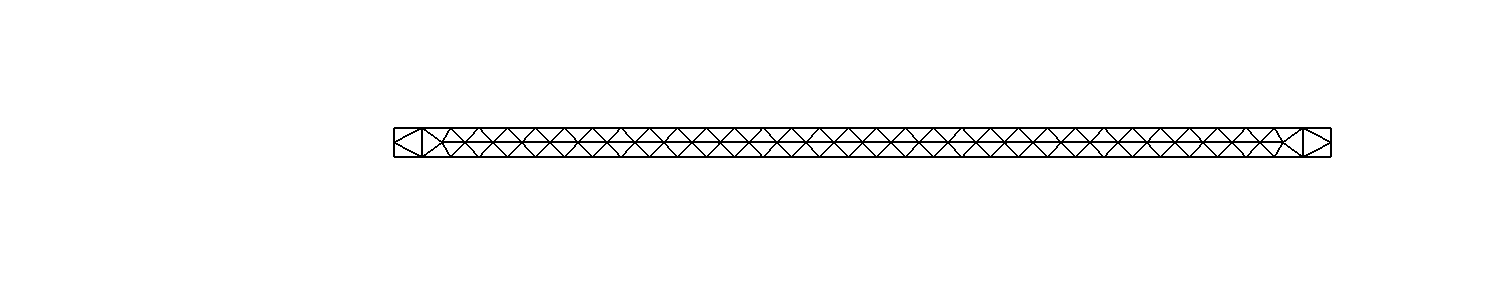
\includegraphics[width=0.92\textwidth]{ch17-mesh-zoom.png}
\end{center}
\begin{itemize}
  \item \code{TRI3} elements: triangles with three nodes, linear shape functions. Three rows of nodes across the thickness ($y = \pm 0.0156$ and $0$), $33$ nodes along each edge, so the triangles' edges are about $0.03$ long: the fine grid spacing $\mathrm{DX} = 2/128 = 0.0156$ times two.
  \item The 2014 slide's rule of thumb: ``Old: mesh edge length $ds = 2\,dx$ (as opposed to $\tfrac12 dx$); new: it seems like $ds = dx$ works better.'' Chapter 18 reconciles this with the \code{MFAC} rule of the examples that build their own mesh; for a read-in mesh the spacing is whatever the file has.
  \item The mesh is made outside IBAMR, in MATLAB's PDE Toolbox, and written in libMesh's \al{MATLAB format} (\code{.mat}, a plain text file; not a MATLAB binary \code{.mat}): slide \ref{fr:matfile}.
\end{itemize}
\sourcecredit{VisIt: the Mesh plot of \code{output.ex2} at $t = 0$, zoomed to the plate.}
\end{frame}

% 9
\begin{frame}[fragile]{The \code{.mat} file, and what libMesh does with it}
\label{fr:matfile}
\footnotesize
The file is numbers separated by spaces: the number of nodes and of elements; then $x\ y$ for each node; then, for each triangle, its three node numbers (counted from 1) and the subdomain number the PDE Toolbox gives it (all $1$ here). The first and last values of \code{IBFE\_Mesh2D\_128.mat}:
\begin{lstlisting}[style=data]
101 130 0.500000 0.015600 0.500000 -0.015600 -0.500000 -0.015600 -0.500000 0.015600 0.500000 0.000000 0.469697 -0.015600 ...
... 41 74 101 1 34 100 101 1
\end{lstlisting}
\begin{itemize}
  \item libMesh's \code{MatlabIO::read\_stream} reads exactly this: ``PDE toolkit only works in 2D'', so the mesh dimension is set to $2$, then \code{nNodes}, \code{nElem}, the coordinates, the connectivity. There is no element-type field: the format is triangles only.
  \item The reader is chosen by the file's extension (slide \ref{fr:formats}); \code{.mat} means ``Matlab triangular ASCII file'' in libMesh's list. Nothing in IBAMR looks inside.
  \item How it was made (the 2016 README's recipe, the only one in the archive): slide \ref{fr:pdetool}.
\end{itemize}
\begin{punchbox}
\footnotesize The four corner nodes come first, then the edges, then the interior: that is the PDE Toolbox's order, and the tutorial's VisIt figures do not depend on it. The order of the four corners you give \code{pdepoly} does matter: the polygon must not cross itself.
\end{punchbox}
\end{frame}

% 10
\begin{frame}[fragile]{Input file: the IBFE-specific lines}
\label{fr:input}
\footnotesize
\begin{lstlisting}[style=inputtiny]
MESH_FILENAME = "IBFE_Mesh2D_128.mat"     // libMesh MATLAB-format mesh of the plate
SHEAR_MODULUS = 10.0                      // shear modulus mu of the neo-Hookean plate
KAPPA_S       = 1.0e6                     // stiffness of the tether force
// MFAC and ELEM_TYPE are used by examples that build their mesh in the program
// (for example IBAMR's IBFE/explicit/ex2). They have no effect on a mesh read
// from a file, like this one. Its element size was chosen when it was made.
MFAC = 2.0                                     // ratio of Lagrangian mesh width to Cartesian mesh width
ELEM_TYPE = "TRI3"                             // type of element to use for structure discretization
PK1_DEV_QUAD_ORDER = "FIFTH"                   // quadrature order for the deviatoric stress
PK1_DIL_QUAD_ORDER = "THIRD"                   // quadrature order for the dilational stress
IB_DELTA_FUNCTION          = "IB_4"            // the type of smoothed delta function to use for Lagrangian-Eulerian interaction
SPLIT_FORCES               = TRUE              // whether to split interior and boundary forces
USE_JUMP_CONDITIONS        = FALSE             // whether to impose pressure jumps at fluid-structure interfaces
USE_CONSISTENT_MASS_MATRIX = TRUE              // whether to use a consistent or lumped mass matrix
IB_POINT_DENSITY           = 2.0               // approximate density of IB quadrature points for Lagrangian-Eulerian interaction

IBFEMethod {
   IB_delta_fcn               = IB_DELTA_FUNCTION
   split_forces               = SPLIT_FORCES
   use_jump_conditions        = USE_JUMP_CONDITIONS
   use_consistent_mass_matrix = USE_CONSISTENT_MASS_MATRIX
   IB_point_density           = IB_POINT_DENSITY
}
Main {
   viz_writer                  = "VisIt","ExodusII"   // VisIt files for the fluid, ExodusII for the plate
   viz_dump_interval           = 100
   viz_dump_dirname            = "viz_IB2d"
   visit_number_procs_per_file = 1
}
\end{lstlisting}
\end{frame}

% 11
\begin{frame}{Input file (2): what each key does}
\label{fr:input2}
\scriptsize
\begin{tabular}{@{}L{0.32\textwidth}L{0.60\textwidth}@{}}
\toprule
key & meaning (from \code{IBFEMethod::getFromInput} in 0.19.0) \\
\midrule
\code{IB\_point\_density} & the approximate number of quadrature points per fine grid cell used to interpolate velocity to and spread force from the elements (the same value for both unless \code{interp\_point\_density} and \code{spread\_point\_density} are given). With \code{use\_adaptive\_quadrature} the rule's order is raised element by element to reach it. More points: no leaks, more cost. \\
\code{IB\_delta\_fcn} & the kernel, as in Part III (\code{IB\_4} here); \code{interp\_delta\_fcn} and \code{spread\_delta\_fcn} can differ. \\
\code{split\_forces} & spread the interior (volumetric) force and the boundary (jump) force separately; sets both \code{split\_normal\_force} and \code{split\_tangential\_force}. \\
\code{use\_jump\_conditions} & impose the pressure jump across the boundary (needs \code{split\_forces}). \\
\code{use\_consistent\_mass\_matrix} & project the interpolated velocity with the consistent mass matrix rather than a lumped one. \\
\bottomrule
\end{tabular}

\end{frame}

% 11b
\begin{frame}{Input file (3): the keys the program reads, and what the old comments got wrong}
\label{fr:input3}
\scriptsize
\begin{tabular}{@{}L{0.32\textwidth}L{0.60\textwidth}@{}}
\toprule
key & meaning \\
\midrule
\code{PK1\_DEV\_QUAD\_ORDER}, \code{PK1\_DIL\_QUAD\_ORDER} & read by \emph{the program}, not by \code{IBFEMethod}, and passed on as each stress function's \code{quad\_order} (slide \ref{fr:register}). \\
\code{MFAC}, \code{ELEM\_TYPE} & read by programs that build their own mesh (\code{ds = MFAC*dx}; the element type); \al{no effect on a mesh read from a file}. The 2014--2024 comments ``It seems like 1.0 is better'' next to \code{MFAC = 2.0} and \code{IB\_POINT\_DENSITY = 2.0} were never acted on; the shipped values are what the runs of slides \ref{fr:full}--\ref{fr:numbers} used. \\
\code{viz\_writer = "VisIt","ExodusII"} & what the examples write; in 0.19.0 the second word is inert: \code{AppInitializer} supplies \code{viz\_IB2d/output.ex2} as the ExodusII file name in any case (the entry only lets an \code{exodus\_filename} key rename it), so the plate file is written whenever \code{viz\_dump\_interval > 0} (checked in chapter 28 with \code{viz\_writer = "VisIt"} alone). \\
\bottomrule
\end{tabular}

\end{frame}

% 12
\begin{frame}[fragile]{The program (1): the start-up, then and now}
\label{fr:startup}
\footnotesize
Current (\code{IBTKInit}, IBAMR 0.10 and later; the example's \code{main.cpp}):
\begin{lstlisting}[style=cpptiny]
int main(int argc, char* argv[])
{
    // Initialize MPI, PETSc, libMesh, SAMRAI and IBAMR. IBTKInit also shuts
    // them down when it goes out of scope at the end of main().
    IBTKInit ibtk_init(argc, argv, MPI_COMM_WORLD);
    const LibMeshInit& init = ibtk_init.getLibMeshInit();
    { // cleanup dynamically allocated objects prior to shutdown
        Pointer<AppInitializer> app_initializer = new AppInitializer(argc, argv, "IB.log");
        Pointer<Database> input_db = app_initializer->getInputDatabase();
\end{lstlisting}
The course versions (2014--2020) did the same by hand, and the 2020 ``main file'' lecture (chapter 23) explains each line:
\begin{lstlisting}[style=cpptiny]
    LibMeshInit init(argc, argv);
    SAMRAI_MPI::setCommunicator(PETSC_COMM_WORLD);
    SAMRAI_MPI::setCallAbortInSerialInsteadOfExit();
    SAMRAIManager::startup();
    ...
    SAMRAIManager::shutdown();
    PetscFinalize();
\end{lstlisting}
\begin{itemize}
  \item \code{IBTKInit(argc, argv, communicator, petsc\_file, petsc\_database)}: the constructor starts MPI, PETSc, SAMRAI and (when IBAMR was built with libMesh) libMesh; the destructor stops them. A second \code{IBTKInit} in the same program is a run-time error.
  \item The old \code{\#include <IBAMR\_config.h>} and \code{<IBTK\_config.h>} are gone; \code{<SAMRAI\_config.h>} stays.
\end{itemize}
\end{frame}

% 13
\begin{frame}[fragile]{The program (2): \code{namespace ModelData}}
\label{fr:modeldata}
\footnotesize
The material and the forces live in a namespace above \code{main()}, as in every IBAMR example. The parameters are static variables that \code{main()} overwrites from the input file:
\begin{lstlisting}[style=cpptiny]
namespace ModelData
{
static const double PI = 3.14159265358979323846;
// Shear modulus of the neo-Hookean plate material, and the stiffness of the
// tether that pulls each point of the plate toward its target position.
// Both can be changed in input2d (SHEAR_MODULUS and KAPPA_S).
static double mu = 10.0;
static double kappa_s = 1.0e6;
// How the target positions move (input key MOTION).
enum class Motion { FULL, HALF, ROTATE };
static Motion motion = Motion::FULL;
...
} // namespace ModelData
using namespace ModelData;
\end{lstlisting}
\begin{itemize}
  \item A namespace, not a class: the callbacks are plain functions (slide \ref{fr:signature}), and IBAMR calls them without any object of yours, so the parameters they need must be visible to them: static variables in the namespace, or a \code{ctx} pointer.
\end{itemize}
\end{frame}

% 13b
\begin{frame}[fragile]{The program (3): \code{main()} reads the model parameters}
\label{fr:modeldata2}
\footnotesize
In \code{main()}, after the input database exists:
\begin{lstlisting}[style=cpptiny]
const string motion_name = input_db->getStringWithDefault("MOTION", "FULL");
if (motion_name == "FULL") ModelData::motion = Motion::FULL;
else if (motion_name == "HALF") ModelData::motion = Motion::HALF;
else if (motion_name == "ROTATE") ModelData::motion = Motion::ROTATE;
else TBOX_ERROR("Unknown MOTION = \"" << motion_name << "\" in the input file.\n" << "Valid options are: FULL, HALF, ROTATE");
ModelData::mu = input_db->getDoubleWithDefault("SHEAR_MODULUS", ModelData::mu);
ModelData::kappa_s = input_db->getDoubleWithDefault("KAPPA_S", ModelData::kappa_s);
\end{lstlisting}
\begin{itemize}
  \item The 2014 version had \code{static const double mu = 10.0; //Elastic modulus of the beam} and \code{kappa\_s = 1.0e6}, fixed in the code. \code{mu} is the shear modulus; \code{ModelData::} is written out in \code{main()} because the fluid's \code{mu} is also in scope there.
\end{itemize}
\end{frame}

% 14
\begin{frame}[fragile]{The callback signature: nine arguments, two namings}
\label{fr:signature}
\footnotesize
Every force or stress function has the shape of \code{IBTK::VectorMeshFcnPtr} (or \code{TensorMeshFcnPtr} for a stress), from \code{libmesh\_utilities.h}:
\begin{lstlisting}[style=cpptiny]
using VectorMeshFcnPtr = void (*)(libMesh::VectorValue<double>& F,          // output: the force (or stress PP)
         const libMesh::TensorValue<double>& FF,                            // deformation gradient dX/ds
         const libMesh::Point& x,                                           // current position
         const libMesh::Point& X,                                           // reference position
         libMesh::Elem* elem,                                               // the element
         const std::vector<const std::vector<double>*>& system_var_data,    // values of registered FE systems
         const std::vector<const std::vector<libMesh::VectorValue<double>>*>& system_grad_var_data,
         double data_time,                                                  // the time
         void* ctx);                                                        // your context pointer
\end{lstlisting}
\begin{tabular}{@{}L{0.22\textwidth}L{0.22\textwidth}L{0.46\textwidth}@{}}
\toprule
IBAMR's name & the course's name & meaning \\
\midrule
\code{x} & \code{X} & where the point is now (current, physical) \\
\code{X} & \code{s} & where it started (reference, Lagrangian); \code{s(0)} is $x$, \code{s(1)} is $y$ \\
\code{FF} & \code{FF} & $\mathbb{F} = \partial\mathbf{X}/\partial\mathbf{s}$, the deformation gradient \\
\code{F} & \code{F} & the output: force per unit reference volume (body force), or $\mathbb{P}$ for a stress function \\
\bottomrule
\end{tabular}

{\scriptsize The course kept Hoover's names (\code{X} current, \code{s} reference) and so does the example; IBAMR's headers use \code{x} and \code{X}. Both are only names. The 2014 slide's seven-argument form with \code{const vector<NumericVector<double>*>\& system\_data} is the pre-2016 signature (slide \ref{fr:legacy}).\par}
\end{frame}

% 15
\begin{frame}[fragile]{The tether force: a target position written in the reference configuration}
\label{fr:tether}
\scriptsize
\begin{columns}[T]
\column{0.5\textwidth}
Chapter 9a's target point: a force $\kappa(\mathbf{X}_{\mathrm{target}} - \mathbf{X})$ toward a prescribed position. Here the prescribed position is a function of where the point started, $\mathbf{s}$, so one formula moves the whole plate. The 2014 slides:

\medskip
``$(\mathbf{s}(0), \mathbf{s}(1))$ are the $(x,y)$ coordinates of the initial mesh. $(\mathbf{s}_{\mathrm{dump}}(0), \mathbf{s}_{\mathrm{dump}}(1))$ are the $(x,y)$ coordinates of where you currently want the target points to be.''

\medskip
Translate up at $V = 0.5$:
\begin{lstlisting}[style=cpptiny]
s_dump(1) = s(1) + 0.5*time;  // only the y-coordinate changes
s_dump(0) = s(0);
\end{lstlisting}
Translate left at $V = 0.3$:
\begin{lstlisting}[style=cpptiny]
s_dump(1) = s(1);
s_dump(0) = s(0) - 0.3*time;  // only the x-coordinate changes
\end{lstlisting}
Then \code{F = kappa\_s*(s\_dump - X)}. Setting \code{s\_dump = X} gives zero force: that is how the plate is released.
\column{0.48\textwidth}
\begin{itemize}
  \item \code{s\_dump} is the course's name for the target position; the example calls it \code{s\_target}.
  \item A slip that survived from 2014 to 2024: the comment ``\code{s(1)} is the x-coordinate of the reference configuration'' on the \code{s\_dump(1)} line. \code{s(1)} is $y$; \code{s(0)} is $x$. (The 2020 deck corrected it on one slide and kept it on two.)
  \item $\kappa_s = 10^6$ is stiff: the plate follows the target to better than $0.01$ (slide \ref{fr:numbers}). $\kappa_s = 10^4$ lags and overshoots.
  \item The force is a \emph{body} force, per unit reference volume, registered with \code{registerLagBodyForceFunction} (slide \ref{fr:register}). It acts on every quadrature point of every element, not only on the nodes.
\end{itemize}
\begin{punchbox}
\footnotesize A moving target in the reference frame is the IBFE way to prescribe motion. Chapter 21's two-coral example and chapter 22's flow tank use the same trick in 3D.
\end{punchbox}
\end{columns}
\end{frame}

% 16
\begin{frame}[fragile]{The tether force (2): the example's one function for all three motions}
\label{fr:tethercode}
\begin{lstlisting}[style=cpptiny]
// Target ("tether") force on the plate, per unit reference area.
//   s is the reference (initial) position of a point in the plate:
//     s(0) is its x-coordinate and s(1) is its y-coordinate.
//   X is where that point is now.
void target_force_function(VectorValue<double>& F, const TensorValue<double>& /*FF*/, const libMesh::Point& X,
                           const libMesh::Point& s, Elem* const /*elem*/,
                           const std::vector<const std::vector<double>*>& /*var_data*/,
                           const std::vector<const std::vector<VectorValue<double> >*>& /*grad_var_data*/,
                           double time, void* /*ctx*/)
{
    libMesh::Point s_target = X;            // the default: no force
    switch (motion)
    {
    case Motion::FULL:
    case Motion::HALF:
        // With HALF, only points that start in the right half (s(0) > 0) are
        // tethered; the left half feels no target force at any time.
        if (motion == Motion::HALF && s(0) <= 0.0) break;
        if (time < 1.0)      { s_target(0) = s(0); s_target(1) = s(1) + 0.5 * time; }               // up at 0.5
        else if (time < 3.0) { s_target(0) = s(0); s_target(1) = s(1) + 0.5 + 0.5 * (1.0 - time); } // down at 0.5
        // for t > 3 the target is X itself: the plate moves only with the fluid
        break;
    // ... continued on the next slide
\end{lstlisting}
\end{frame}

% 16b
\begin{frame}[fragile]{The tether force (3): the ROTATE case and the force}
\label{fr:tethercode2}
\begin{lstlisting}[style=cpptiny]
    case Motion::ROTATE:
        if (time < 1.0)
        {   // turn counterclockwise about the origin by a quarter turn over 0 < t < 1
            const double theta = 0.5 * PI * time;
            s_target(0) = s(0) * std::cos(theta) - s(1) * std::sin(theta);
            s_target(1) = s(0) * std::sin(theta) + s(1) * std::cos(theta);
        }
        break;                              // for t > 1 the plate is released
    }
    F = kappa_s * (s_target - X);
}
\end{lstlisting}
\footnotesize
\begin{itemize}
  \item The \code{switch} replaces the course's three programs: one function, one input key. \code{s\_target = X} before the \code{switch} is the ``no force'' default that every released or untethered point falls through to.
  \item \code{F} is the force per unit reference area (2D) or volume (3D) at the point; IBAMR multiplies by the element's quadrature weights and spreads it.
\end{itemize}
\end{frame}

% 17
\begin{frame}[fragile]{FULL and HALF: the 2014 code, side by side with the example's}
\label{fr:halfcode}
\footnotesize
\begin{columns}[T]
\column{0.5\textwidth}
Hoover's \code{TetherForceFullPlate2D} (2014, slide 12):
\begin{lstlisting}[style=cpptiny]
libMesh::Point s_dump;   //s_dump is the target point position
if(time<1)  //move the beam up with a speed of 0.5 from 0<t<1
{
  s_dump(1)=s(1)+.5*time;
  s_dump(0)=s(0);
}
else if(time<3)  //move the beam down with a speed of -0.5 for 1<t<3
{
  s_dump(1)=s(1)+.5+.5*(1-time);
  s_dump(0)=s(0);
}
else  //set the target point location to the actual location
{     //of the boundary (X) to make force equal to zero.
  s_dump(1)=X(1);
  s_dump(0)=X(0);
}
F = kappa_s*(s_dump-X);
return;
\end{lstlisting}
\column{0.48\textwidth}
\code{TetherForceHalfPlate2D} (2014, slide 14): ``This if statement only applies a force if you are on the right side.''
\begin{lstlisting}[style=cpptiny]
if(s(0)>0){
  libMesh::Point s_dump;
  if(time<1) { s_dump(1)=s(1)+.5*time; s_dump(0)=s(0); }
  else if(time<3){ s_dump(1)=s(1)+.5+.5*(1-time); s_dump(0)=s(0); }
  else{ s_dump(1)=X(1); s_dump(0)=X(0); }
  F = kappa_s*(s_dump-X);
}
else{
  F.zero();   //Else the force is set to zero.
}
return;
\end{lstlisting}
\end{columns}
\end{frame}

% 17b
\begin{frame}{FULL and HALF (2): what the two versions share}
\label{fr:halfcode2}
\footnotesize
\begin{itemize}
  \item \code{F.zero()} and \code{F = kappa\_s*(X - X)} are the same force. The example's \code{s\_target = X} default and the early \code{break} fold the three versions into one \code{switch}.
  \item ``The movement of the other half of the plate is purely passive (i.e.\ PK1 stress)'': the left half is carried by the material law alone. That is why the plate bends (slide \ref{fr:half}).
  \item The 2014 deck placed the centre of the plate at the origin, so \code{s(0) > 0} is the right half; the mesh file confirms it ($x \in [-0.5, 0.5]$).
  \item The 2014 text for the half plate: ``Again using a body force acting as tether force defined in the ModelData namespace, I now have half the plate move up to $.5$ (in 1 s) then down $1.0$ (in 2 s), after which I turn off the force (for 1 s).''
\end{itemize}
\end{frame}

% 18
\begin{frame}[fragile]{ROTATE: a rotation that was only a rotation on the centre line}
\label{fr:rotatecode}
\footnotesize
\begin{columns}[T]
\column{0.5\textwidth}
Hoover's \code{TetherForceFullPlate2D-Rotate} (2014, slide 17; unchanged through 2024):
\begin{lstlisting}[style=cpptiny]
if(time<1)
{
  s_dump(1)=s(1)+s(0)*sin(2*3.14*0.5*time);  //y-coordinate gets moved
                 //more the farther along the beam you are
  //should really define PI here
  s_dump(0)=s(0)*cos(2*3.14*0.5*time); //adjustment for x-coordinate
}
else //turns off all forcing, target coordinates set to current
{
  s_dump(1)=X(1);
  s_dump(0)=X(0);
}
F = kappa_s*(s_dump-X);
\end{lstlisting}
With $\theta = 2\cdot 3.14\cdot 0.5\,t \approx \pi t$: a half turn in one second, and
\[ x' = x\cos\theta,\qquad y' = y + x\sin\theta . \]
\column{0.48\textwidth}
The example's version (slide \ref{fr:tethercode2}), with $\theta = \pi t/2$:
\begin{lstlisting}[style=cpptiny]
const double theta = 0.5 * PI * time;
s_target(0) = s(0) * std::cos(theta) - s(1) * std::sin(theta);
s_target(1) = s(0) * std::sin(theta) + s(1) * std::cos(theta);
\end{lstlisting}
\[ x' = x\cos\theta - y\sin\theta,\qquad y' = x\sin\theta + y\cos\theta . \]
The 2014 and 2020 text: ``The goal here is to spin the beam about its center for $t<1$, and then release it.''
\end{columns}
\end{frame}

% 18b
\begin{frame}{ROTATE (2): what the old formula did, and what the example does}
\label{fr:rotatecode2}
\footnotesize
\begin{itemize}
  \item A rotation by $\theta$ is $x' = x\cos\theta - y\sin\theta$, $y' = x\sin\theta + y\cos\theta$. The 2014 formula drops $-y\sin\theta$ and replaces $y\cos\theta$ by $y$: exact for $y = 0$ (the centre line), and off by up to the plate's half-thickness, $0.0156$, elsewhere. With $\kappa_s = 10^6$ the plate was pulled into a slightly sheared shape, not a rotated one.
  \item $2\cdot 3.14$ for $2\pi$ (``should really define PI here'') is a $0.05$ per cent error in the angle; the example defines \code{PI} to full precision.
  \item The 2014 text said ``spin the beam about its center for $t < 1$'', the formula gives a half turn ($\theta(1) = \pi$); the 2020 and 2024 decks said the same. The example makes it a quarter turn ($\theta = \pi t/2$) so that the released plate's drift is visible against the start (slide \ref{fr:rotate}); set \code{theta = PI * time} for the half turn.
  \item The target of a point at the origin never moves, so the centre of the plate stays put: the measurement on slide \ref{fr:numbers} confirms it to three digits.
\end{itemize}
\end{frame}

% 19
\begin{frame}[fragile]{The fourth 2014 example: a sinusoidal body force on the plate's ends}
\label{fr:sinus}
\scriptsize
The 2014 deck's slide 15, ``\code{Example\_IBFE\_SinusoidalForce2D}'': ``Here I define a body force that is sinusoidally forcing our plate. The forced elements lie between $-0.25$ to $0.25$ on the horizontal axis of the reference configuration.'' The code was never on a slide, and the 2018 and later decks dropped it; the folder survives as \code{Example\_IBFE\_SinusoidalForce2D\_2016-11.zip} in the course's 2016-11 example set, and its \code{main.C} (2017-02-09) forces the \emph{outer} quarters, \code{abs(s(0)) > .25}, not the middle half the slide describes:
\begin{lstlisting}[style=cpptiny]
static const double mu = 10.0;
static double kappa_s = 3.0e1;          // the force amplitude, per unit reference area
static const double freq = 0.5;         // half a cycle per unit time
static const double PI = acos(-1);
void sinusoidal_force_function(VectorValue<double>& F, const TensorValue<double>& /*FF*/, const libMesh::Point& X,
                               const libMesh::Point& s, Elem* const /*elem*/,
                               const vector<NumericVector<double>*>& /*system_data*/, double time, void* /*ctx*/)   // the 2016 signature
{
  if(abs(s(0)) >.25){
  libMesh::Point s_dump;
  s_dump(0)=0;
  s_dump(1)=1;                          // a unit vector up
  F = kappa_s*sin(2*PI*time*freq)*s_dump;
} else{
  F.zero();
 }
    return;
}
\end{lstlisting}
\end{frame}

% 19b
\begin{frame}{The fourth 2014 example (2): what the code does, and how to run it today}
\label{fr:sinus2}
\footnotesize
\begin{itemize}
  \item A vertical force $30\sin(\pi t)$ per unit reference area on the two ends, nothing on the middle: the ends flap up and down and the free middle follows through the material law. The variable names are the tether's (\code{kappa\_s}, \code{s\_dump}) reused for an amplitude and a direction; the slide's ``between $-0.25$ and $0.25$'' is the complement of what the code does.
  \item The plate has no tether here, so this is the one course example where the plate is free and driven by a body force alone; chapter 19 returns to it. To run it today: the nine-argument signature, \code{std::abs}, and \code{LagBodyForceFcnData} as on slide \ref{fr:register}; only one body force function can be registered per part (the header: ``It is \emph{NOT} possible to register multiple body force functions with this class''), so a plate that is both tethered and shaken needs both terms in one function. Exercise 2 (slide \ref{fr:exercises}) is to run it.
\end{itemize}
\end{frame}

% 20
\begin{frame}[fragile]{The stress functions: a neo-Hookean plate in two parts}
\label{fr:pk1}
\footnotesize
\begin{lstlisting}[style=cpptiny]
// Stress tensor functions. The first Piola-Kirchhoff stress of the neo-Hookean
// material is split into two parts. The deviatoric part is mu*FF. The
// dilational part, -mu*FF^{-T}, makes the undeformed plate stress-free: at
// FF = I the two parts cancel.
void PK1_dev_stress_function(TensorValue<double>& PP, const TensorValue<double>& FF, const libMesh::Point& /*X*/,
                             const libMesh::Point& /*s*/, Elem* const /*elem*/,
                             const std::vector<const std::vector<double>*>& /*var_data*/,
                             const std::vector<const std::vector<VectorValue<double> >*>& /*grad_var_data*/,
                             double /*time*/, void* /*ctx*/)
{
    PP = mu * FF;
}
void PK1_dil_stress_function(TensorValue<double>& PP, const TensorValue<double>& FF, ...same arguments...)
{
    PP = -mu * tensor_inverse_transpose(FF, NDIM);
}
\end{lstlisting}
\begin{itemize}
  \item $\mathbb{P} = \mu\,\mathbb{F} - \mu\,\mathbb{F}^{-T}$: the 2014 slide's ``Neo-Hookean model: think springs''. At $\mathbb{F} = \mathbb{I}$ the two parts cancel, so the plate as meshed carries no stress; stretch it and $\mu\mathbb{F}$ pulls back.
  \item Why two functions: IBAMR integrates each registered stress with its own quadrature rule. The smooth deviatoric part gets \code{PK1\_DEV\_QUAD\_ORDER = "FIFTH"}, the inverse-transpose part \code{"THIRD"}; chapter 19 explains the choice and the other material laws (and corrects the 2014 claim that $-\mu\mathbb{F}^{-T}$ ``enforces incompressibility'': it does not, it only makes the reference state stress-free).
  \item \code{tensor\_inverse\_transpose(FF, NDIM)} is IBAMR's helper from \code{libmesh\_utilities.h}; \code{mu} is \code{ModelData::mu}, the shear modulus.
\end{itemize}
\end{frame}

% 21
\begin{frame}[fragile]{Registering the functions}
\label{fr:register}
\footnotesize
\begin{lstlisting}[style=cpptiny]
// Configure the IBFE solver: register the stress and force functions,
// then set up the finite element systems.
IBFEMethod::LagBodyForceFcnData target_force_data(target_force_function);
IBFEMethod::PK1StressFcnData PK1_dev_stress_data(PK1_dev_stress_function);
IBFEMethod::PK1StressFcnData PK1_dil_stress_data(PK1_dil_stress_function);
PK1_dev_stress_data.quad_order = Utility::string_to_enum<libMesh::Order>(input_db->getStringWithDefault("PK1_DEV_QUAD_ORDER", "THIRD"));
PK1_dil_stress_data.quad_order = Utility::string_to_enum<libMesh::Order>(input_db->getStringWithDefault("PK1_DIL_QUAD_ORDER", "FIRST"));
ib_method_ops->registerPK1StressFunction(PK1_dev_stress_data);
ib_method_ops->registerPK1StressFunction(PK1_dil_stress_data);
ib_method_ops->registerLagBodyForceFunction(target_force_data);
ib_method_ops->initializeFEEquationSystems();
EquationSystems* equation_systems = ib_method_ops->getFEDataManager()->getEquationSystems();
\end{lstlisting}
\begin{itemize}
  \item A \code{*FcnData} struct wraps each function pointer with an optional \code{ctx} pointer and the list of FE systems whose values the function wants (\code{system\_data}; chapter 20 uses it for the fibre direction). The stress structs also carry the quadrature rule.
  \item \code{initializeFEEquationSystems()} must come after the registrations and before \code{initializeFEData()}.
\end{itemize}
\end{frame}

% 21b
\begin{frame}{Registering the functions (2): the data structs, and how many of each}
\label{fr:register2}
\footnotesize
\begin{tabular}{@{}L{0.30\textwidth}L{0.62\textwidth}@{}}
\toprule
struct (in \code{FEMechanicsBase}) & fields, and how many per part \\
\midrule
\code{PK1StressFcnData} & \code{fcn}, \code{system\_data}, \code{ctx}, \code{quad\_type}, \code{quad\_order}; \al{any number} (each call \code{push\_back}s; a missing \code{quad\_order} takes the part's default) \\
\code{LagBodyForceFcnData} & \code{fcn}, \code{system\_data}, \code{ctx}; \al{one} (a second call replaces the first) \\
\code{LagSurfacePressureFcnData}, \code{LagSurfaceForceFcnData} & \code{fcn}, \code{system\_data}, \code{ctx}; \al{one} each (slide \ref{fr:surface}) \\
\code{CoordinateMappingFcnData} & \code{fcn}, \code{ctx}: initial physical position from the reference position (chapter 22's translated mesh) \\
\code{InitialVelocityFcnData} & \code{fcn}, \code{ctx}: a starting velocity for the solid (zero if none) \\
\bottomrule
\end{tabular}

\medskip
The second argument of every \code{register*} call is the part number (default $0$); with several meshes (chapter 21) each part has its own functions. \code{libMesh::Order} replaced the course's \code{libMeshEnums::Order} in 2016.
\end{frame}

% 22
\begin{frame}[fragile]{Surface forces and pressures: listed in every version, shown in none}
\label{fr:surface}
\footnotesize
The 2014 slide 3 listed ``Body Force, Surface Force''; no course deck ever showed one. They act on the \emph{boundary} of the mesh (per unit reference area) and have twelve arguments: the nine of slide \ref{fr:signature} plus the current and reference normals and the side of the element:
\begin{lstlisting}[style=cpptiny]
using ScalarSurfaceFcnPtr = void (*)(
         double& F,                                   // output: a pressure p (the force is -p n)
         const libMesh::VectorValue<double>& n,       // current unit normal
         const libMesh::VectorValue<double>& N,       // reference unit normal
         const libMesh::TensorValue<double>& FF,      // deformation gradient
         const libMesh::Point& x,                     // current position
         const libMesh::Point& X,                     // reference position
         libMesh::Elem* elem,                         // the element
         unsigned short int side,                     // which of its sides
         const std::vector<const std::vector<double>*>& system_var_data,
         const std::vector<const std::vector<libMesh::VectorValue<double>>*>& system_grad_var_data,
         double data_time,
         void* ctx);
// VectorSurfaceFcnPtr: the same, with libMesh::VectorValue<double>& F (a force vector) as the output
\end{lstlisting}
\end{frame}

% 22b
\begin{frame}[fragile]{Surface forces and pressures (2): a pressure load, and when to use which}
\label{fr:surface2}
\footnotesize
A pressure load $p_0$ on every boundary side of the plate, and its registration:
\begin{lstlisting}[style=cpptiny]
void surface_pressure_function(double& P,
                               const VectorValue<double>& /*n*/, const VectorValue<double>& /*N*/,
                               const TensorValue<double>& /*FF*/,
                               const libMesh::Point& /*x*/, const libMesh::Point& /*X*/,
                               Elem* const /*elem*/, const unsigned short int /*side*/,
                               const std::vector<const std::vector<double>*>& /*var_data*/,
                               const std::vector<const std::vector<VectorValue<double> >*>& /*grad_var_data*/,
                               double /*time*/, void* /*ctx*/)
{
    P = 1.0;
}
IBFEMethod::LagSurfacePressureFcnData surface_pressure_data(surface_pressure_function);
ib_method_ops->registerLagSurfacePressureFunction(surface_pressure_data);
\end{lstlisting}
\begin{itemize}
  \item Use a surface pressure for a load that acts on a face (an inflating tube, a transmural pressure); a surface force for a traction with a direction of its own. Restrict either with \code{side} or with the reference position \code{X}. Chapter 23 shows the upstream examples that use them.
\end{itemize}
\end{frame}

% 23
\begin{frame}[fragile]{Reading your mesh}
\label{fr:readmesh}
\footnotesize
\begin{lstlisting}[style=cpptiny]
// Read the finite element mesh of the plate. The .mat format is
// libMesh's MATLAB mesh format (see README.md for how it was made).
Mesh mesh(init.comm(), NDIM);
mesh.read(input_db->getStringWithDefault("MESH_FILENAME", "IBFE_Mesh2D_128.mat"));
mesh.prepare_for_use();
\end{lstlisting}
\begin{itemize}
  \item \code{Mesh mesh(init.comm(), NDIM)}: a libMesh mesh on the communicator \code{IBTKInit} made, of dimension \code{NDIM} ($2$ for \code{main2d}). The 2014 slide shows \code{Mesh mesh(NDIM)} ``for \code{ibamr/3803}'' and the communicator form ``for \code{ibamr/2016-11}''; only the second compiles today.
  \item \code{mesh.read(name)} chooses the reader from the extension (next slide) and fills the mesh; \code{prepare\_for\_use()} builds the neighbour and boundary information every later step needs. Call it once, after reading.
  \item The 2014 slide also read \code{DX}, \code{ds = MFAC*dx} and \code{ELEM\_TYPE} here; for a mesh from a file they are unused, and the example does not read them (the input keeps them, commented, for the programs that do).
  \item The mesh is then handed to the method: \code{new IBFEMethod("IBFEMethod", db, \&mesh, max\_levels, register\_for\_restart, restart\_read\_dirname, restart\_restore\_num)}, and \code{ib\_method\_ops->initializeFEData()} after the registrations.
\end{itemize}
\begin{punchbox}
\footnotesize ``Look at the README files in the examples'' (2014). The READMEs are in \code{examples/IBFE/*/README.md} and say, for each example, where its mesh came from.
\end{punchbox}
\end{frame}

% 24
\begin{frame}{Mesh formats libMesh reads (by file extension)}
\label{fr:formats}
\footnotesize
\begin{tabular}{@{}L{0.16\textwidth}L{0.40\textwidth}L{0.36\textwidth}@{}}
\toprule
extension & format (libMesh 1.7.8, \code{NameBasedIO}) & used in this tutorial by \\
\midrule
\code{.mat} & MATLAB triangular ASCII (PDE Toolbox) & IBFE/01, 06, 12 \\
\code{.msh} & gmsh (ASCII versions 2.2 and 4; never binary) & IBFE/05 triangle, IBFE/10 3D plate; chapter 18 \\
\code{.e}, \code{.exo}, \code{.exd} & ExodusII (also what IBAMR writes) & IBFE/08 beam and circle; Coreform Cubit exports \\
\code{.node} + \code{.ele} & TetGen (3D) and Triangle (2D) & chapter 18 \\
\code{.inp} & Abaqus & -- \\
\code{.ucd}, \code{.unv}, \code{.gmv}, \code{.off}, \code{.mesh} & AVS UCD, I-deas Universal, General Mesh Viewer, OOGL OFF, Medit & -- \\
\code{.vtu} & VTK unstructured (Paraview) & -- \\
\code{.xda}, \code{.xdr} & libMesh's own ASCII and binary formats & \code{output\_data()} writes \code{fe\_mesh.*.xda} \\
\code{.cpa}, \code{.cpr} & libMesh checkpoint, ASCII and binary & -- \\
\bottomrule
\end{tabular}

\medskip
\begin{itemize}
  \item The list is printed by libMesh itself when it does not recognise an extension (\code{NameBasedIO::read}: ``ERROR: Unrecognized file extension'' followed by the formats).
  \item Writing goes through the same class: \code{mesh.write("plate.e")} converts a \code{.mat} mesh to ExodusII, which VisIt can open on its own (chapter 28).
  \item The 2014 deck's ``There are many other options (look at the libmesh MeshInput link)'' is this table.
\end{itemize}
\end{frame}

% 25
\begin{frame}[fragile]{The rest of \code{main()}: what is new for IBFE, what is chapter 5's}
\label{fr:restofmain}
\scriptsize
\begin{tabular}{@{}L{0.44\textwidth}L{0.48\textwidth}@{}}
\toprule
line & what it does \\
\midrule
\code{new IBFEMethod("IBFEMethod", db, \&mesh,}\newline\code{max\_levels, true, restart\_read\_dirname,}\newline\code{restart\_restore\_num)} & the IB operations for the mesh; \code{register\_for\_restart = true} so that the mesh data goes into the restart files \\
\code{new IBExplicitHierarchyIntegrator(...,}\newline\code{ib\_method\_ops, navier\_stokes\_integrator)} & the same time integrator as the IB examples; it does not care which \code{IBStrategy} it drives \\
\code{initializeFEEquationSystems();}\newline\code{getFEDataManager()->getEquationSystems()} & create the FE systems (position, velocity, force) on the mesh; the \code{EquationSystems} pointer is what the ExodusII writer writes \\
\code{std::unique\_ptr<ExodusII\_IO> exodus\_io =}\newline\code{uses\_exodus ? std::make\_unique<ExodusII\_IO>(mesh)}\newline\code{: nullptr;} & the plate's output file writer (libMesh); the course used \code{AutoPtr}, removed from libMesh in 2017 \\
\code{exodus\_io->append(from\_restart);} & a restarted run adds its steps to the existing \code{output.ex2} instead of starting it over \\
\bottomrule
\end{tabular}

\end{frame}

% 25b
\begin{frame}[fragile]{The rest of \code{main()} (2): output, restart, post-processing}
\label{fr:restofmain2}
\scriptsize
\begin{tabular}{@{}L{0.44\textwidth}L{0.48\textwidth}@{}}
\toprule
line & what it does \\
\midrule
\code{initializeFEData();}\newline\code{initializePatchHierarchy(...)} & FE data first, then the fluid grid \\
\code{exodus\_io->write\_timestep(exodus\_filename,}\newline\code{*equation\_systems,}\newline\code{iteration\_num / viz\_dump\_interval + 1, loop\_time);} & one time state per visualization dump, numbered from $1$ \\
\code{writeFEDataToRestartFile(}\newline\code{restart\_dump\_dirname, iteration\_num)} & next to the SAMRAI restart file: both are needed to restart \\
\code{output\_data(...)}: \code{mesh.write(fe\_mesh.NNNNN.xda)},\newline\code{equation\_systems->write(...)} & the post-processing dump (\code{data\_dump\_interval > 0}): the mesh and all FE data in libMesh's own format \\
\bottomrule
\end{tabular}

\medskip
The fluid solver choice, the initial and boundary condition objects, the \code{VisItDataWriter}, the time loop and the restart and timer dumps are the chapter 5 program line for line.
\end{frame}

% 26
\begin{frame}[fragile]{Build and run}
\label{fr:build}
\footnotesize
\begin{lstlisting}[style=shell]
module load gnu13 openmpi5                       # Puma only; a laptop with autoibamr skips this line
source ~/autoibamr/configuration/enable.sh
cmake -S . -B build -DCMAKE_BUILD_TYPE=Release
cmake --build build -j 4
mpirun -np 4 ./build/main2d input2d              # or: sbatch job.slurm
\end{lstlisting}
\begin{itemize}
  \item \code{CMakeLists.txt} is the six-line file of chapter 3 (\code{find\_package(IBAMR 0.16.0 REQUIRED)}, \code{target\_link\_libraries(main2d PRIVATE IBAMR::IBAMR2d)}); libMesh comes with IBAMR's targets, nothing to add. The 2014 Makefile needed \code{LIBSNEW = \$(LIBS) -lnetcdf -lcurl} by hand (slide \ref{fr:legacy}).
  \item $4000$ steps of \code{DT = 1e-3} to $t = 4$; $41$ visualization dumps; $26$ s on four laptop cores with 0.16.0, about the same with 0.19.0. The two versions give the same positions to three digits.
  \item A misspelled \code{MOTION} stops the run at once:
\end{itemize}
\begin{lstlisting}[style=data]
Unknown MOTION = "ROTATE2" in the input file.
Valid options are: FULL, HALF, ROTATE
\end{lstlisting}
\begin{itemize}
  \item Two course-era traps, fixed in the shipped files: the half-plate and rotate input files ended with a stray \code{\textbackslash\textbackslash} (an input parse error at start-up), and a file saved with Windows line endings stops with \code{Illegal character token in input} (chapter 6). The course hid the second by ending every line with \code{//}.
\end{itemize}
\end{frame}

% 27
\begin{frame}{The output: two kinds of files}
\label{fr:output}
\footnotesize
\begin{tabular}{@{}L{0.26\textwidth}L{0.66\textwidth}@{}}
\toprule
\code{viz\_IB2d/dumps.visit} & the fluid on the adaptive grid, as in Part III: \code{U}, \code{P}, \code{Omega}, \code{F} (the spread force), \code{Div\_U}, one \code{visit\_dump.NNNNN} folder per dump \\
\code{viz\_IB2d/output.ex2} & the plate, one ExodusII file with all $41$ time states: the mesh (\code{Mesh}, one element block, node numbers) and the nodal variables \code{dX\_0}, \code{dX\_1} (displacement from the reference position), \code{X\_0}, \code{X\_1} (current position), \code{F\_0}, \code{F\_1} (force) and \code{U\_0}, \code{U\_1} (velocity) \\
\code{IB.log}, \code{IB2d.log} & the log (\code{AppInitializer}'s name in the program; \code{log\_file\_name} in \code{Main}) \\
\code{restart\_IB2d/} & only with \code{restart\_dump\_interval > 0}: SAMRAI's files and \code{writeFEDataToRestartFile}'s \\
\code{hier\_data\_IB2d/} & only with \code{data\_dump\_interval > 0}: \code{hier\_data.NNNNN.samrai.PPPPP} (HDF5), \code{fe\_mesh.NNNNN.xda}, \code{fe\_equation\_systems.NNNNN} \\
\bottomrule
\end{tabular}

\begin{itemize}
  \item ``\code{dumps.visit}: Eulerian data; \code{output.ex2}: finite element / Lagrangian data; Exodus II type file; can have multiple files of this type for different parts of object'' (2014). With several meshes (chapter 21) IBAMR writes one \code{.ex2} per part.
  \item There is no \code{lag\_data.visit} here: the plate is not a point set. VisIt reads ExodusII directly (next slides), and so do Python (\code{netCDF4}, \code{exodus.py}) and MATLAB (\code{ncread}); chapter 28 reads the positions of the tips from it.
  \item The 2020 deck wrote ``\code{dump.visit}''; the file is \code{dumps.visit}.
\end{itemize}
\end{frame}

% 28
\begin{frame}{Seeing the plate in VisIt: the mesh is drawn where it started}
\label{fr:visit1}
\footnotesize
\begin{columns}[T]
\column{0.5\textwidth}
\begin{center}
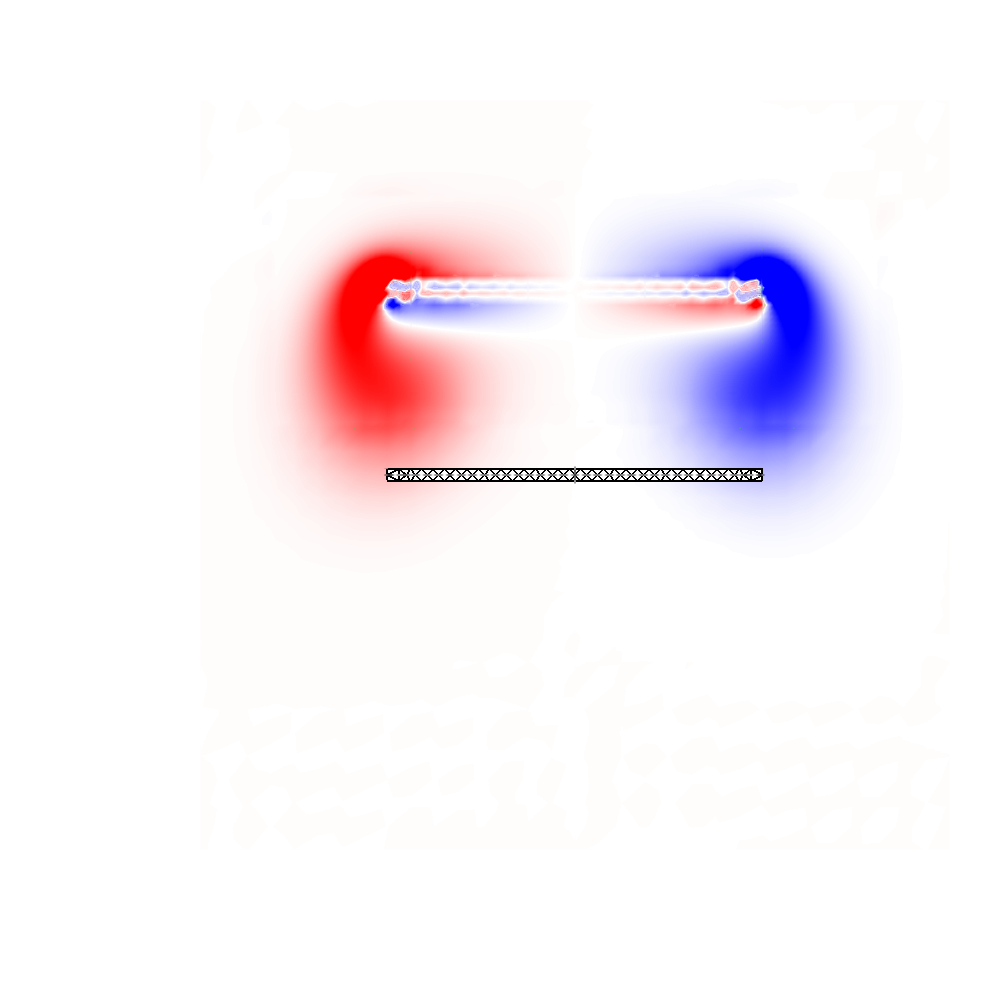
\includegraphics[height=0.62\textheight]{ch17-full-t1-nodisplace.png}
\end{center}
\column{0.48\textwidth}
\begin{enumerate}
  \item Open \code{viz\_IB2d/dumps.visit}; \textbf{Add $\to$ Pseudocolor $\to$ Omega}; \textbf{Draw}.
  \item Open \code{viz\_IB2d/output.ex2} as a second source; \textbf{Add $\to$ Mesh $\to$ Mesh}; \textbf{Draw}.
  \item Untick \textbf{Apply operators to all plots} (bottom left of the plot list), so that the next step touches only the mesh plot.
\end{enumerate}
At $t = 1$ the vorticity shows the plate has moved up by $0.5$, but the mesh is drawn at its \emph{starting} position: ExodusII stores the reference mesh and the displacement \code{dX} separately. The next slide moves it.
\begin{punchbox}
\footnotesize The 2014 README and every deck since teach this with a YouTube video by Shannon Jones (\code{watch?v=Kj\_MACemSd0}); the IBFE Read Me adds ``the youtube tutorial has a mistake, but this is corrected in the google slides.'' The video is listed in chapter 0.1 and not reproduced.
\end{punchbox}
\end{columns}
\end{frame}

% 29
\begin{frame}{Seeing the plate in VisIt (2): the \code{dX} expression and the Displace operator}
\label{fr:visit2}
\footnotesize
\begin{columns}[T]
\column{0.5\textwidth}
\begin{center}
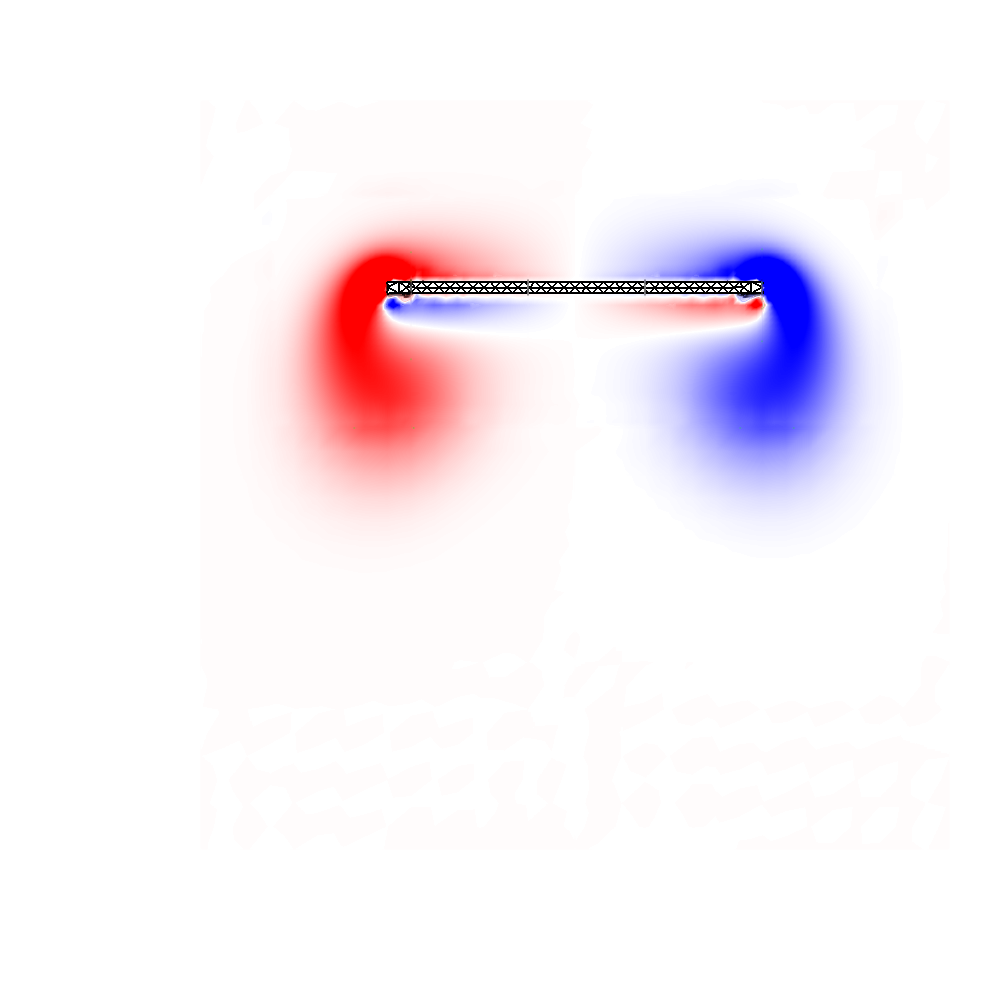
\includegraphics[height=0.62\textheight]{ch17-full-t1.png}
\end{center}
\column{0.48\textwidth}
\begin{enumerate}
  \setcounter{enumi}{3}
  \item \textbf{Controls $\to$ Expressions $\to$ New}: name \code{dX}, type \emph{Vector Mesh Variable}, definition \code{\{dX\_0, dX\_1\}}; \textbf{Apply}.
  \item Select the Mesh plot; \textbf{Operators $\to$ Transforms $\to$ Displace}; in its attributes set \emph{Displacement variable} to \textbf{Vectors $\to$ dX}; \textbf{Apply}; \textbf{Draw}.
  \item Save the expression (\textbf{Expressions $\to$ Save} writes an XML file) or the whole session; you will do this for every IBFE run.
\end{enumerate}
\end{columns}
\end{frame}

% 29b
\begin{frame}{Seeing the plate in VisIt (3): older output, 3D, and what chapter 28 adds}
\label{fr:visit3}
\footnotesize
\begin{itemize}
  \item Older IBAMR versions wrote the 2D mesh with three coordinates: then the definition was \code{\{dX\_0, dX\_1, 0\}} and the mesh had to be flattened with \textbf{Operators $\to$ Transforms $\to$ Project} (``the default projection should be for the xy-plane''). Current output is two-dimensional (\code{coordx}, \code{coordy} only), so \code{\{dX\_0, dX\_1\}} and no Project, as the 2020 note ``for new ibamr install in 2D'' says.
  \item In 3D the expression is \code{\{dX\_0, dX\_1, dX\_2\}}.
  \item Chapter 28 continues: colouring the mesh by \code{F} or \code{U}, picking nodes, the scripted version.
  \item The figures of this chapter were made the scripted way (\code{wsl/final/visit\_ch17.sh}): \code{DefineVectorExpression("dX", "\{dX\_0, dX\_1\}")}, \code{AddPlot("Mesh", "Mesh")}, \code{AddOperator("Displace")} with \code{DisplaceAttributes().variable = "dX"}. Chapter 32 has the whole recipe.
\end{itemize}
\end{frame}

% 30
\begin{frame}{FULL: up, down, released}
\label{fr:full}
\begin{columns}[T]
\column{0.25\textwidth}\centering 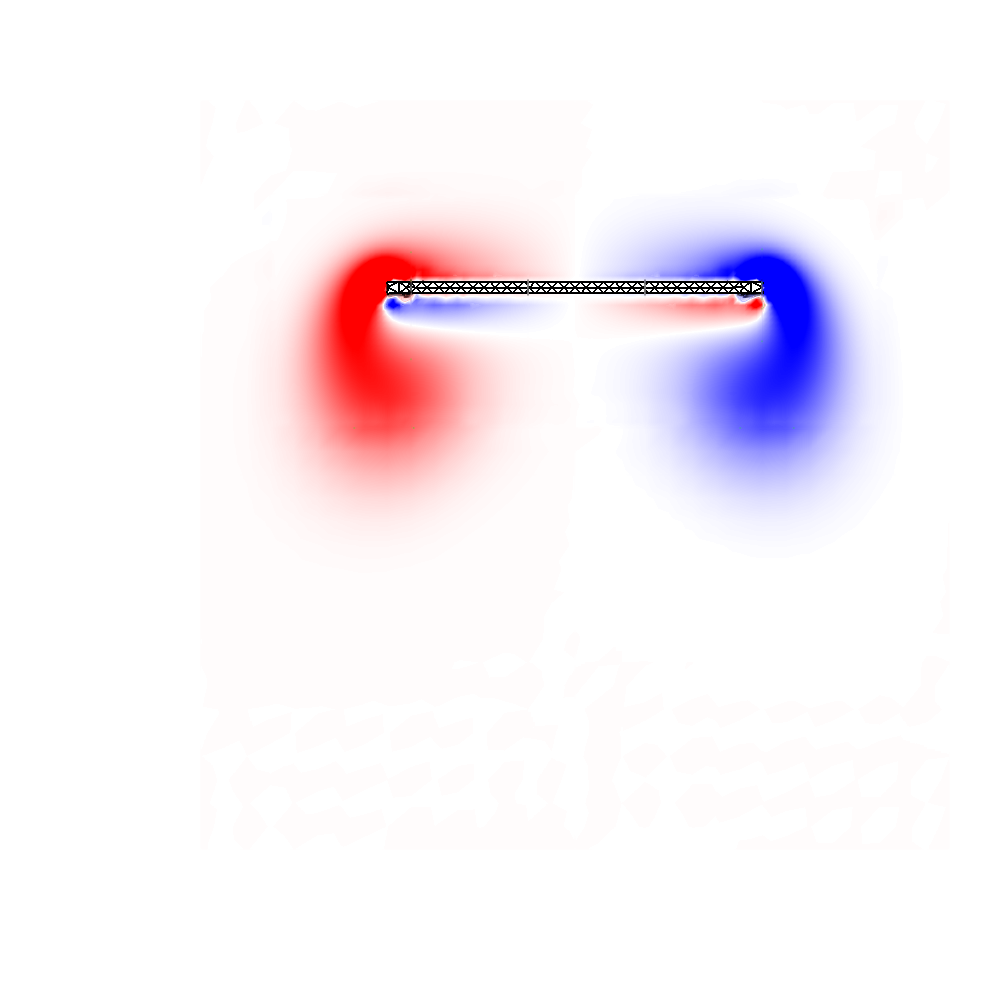
\includegraphics[width=\textwidth]{ch17-full-t1.png}\\ \scriptsize $t = 1$: top of the motion
\column{0.25\textwidth}\centering 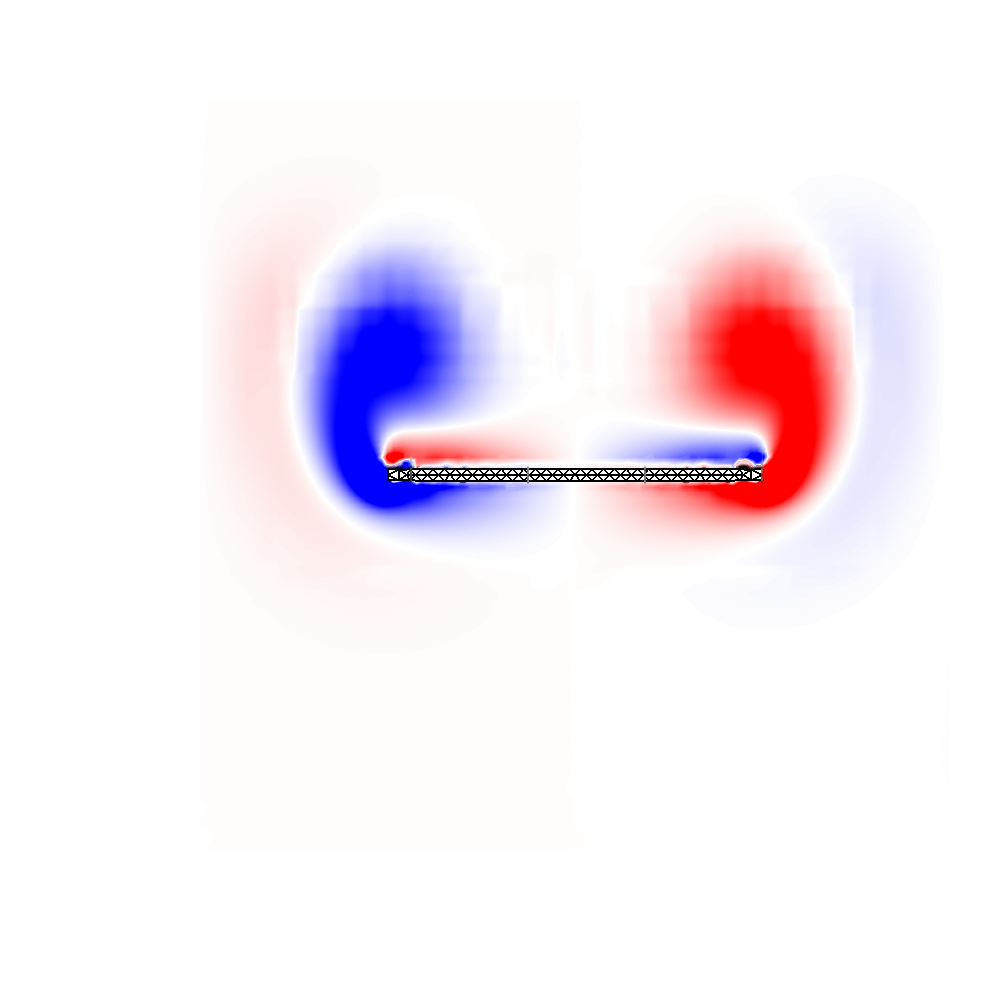
\includegraphics[width=\textwidth]{ch17-full-t2.png}\\ \scriptsize $t = 2$: on the way down
\column{0.25\textwidth}\centering 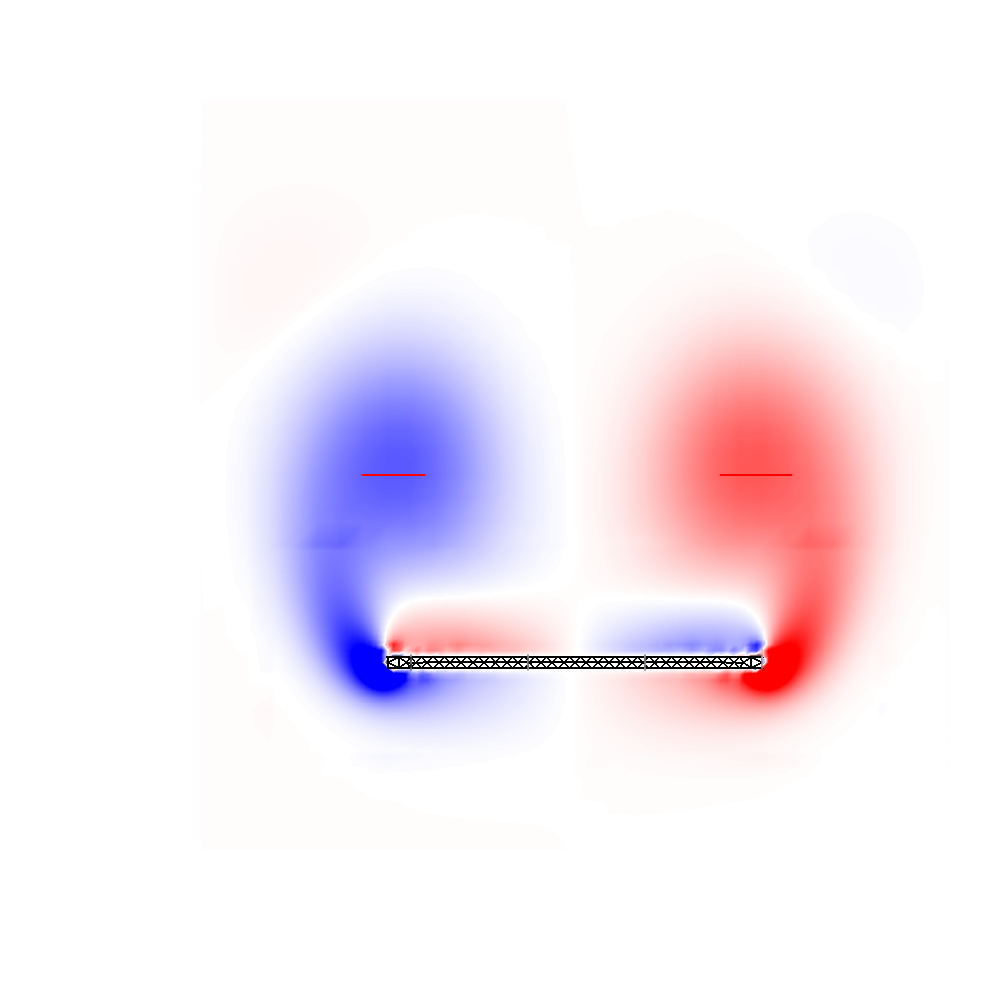
\includegraphics[width=\textwidth]{ch17-full-t3.png}\\ \scriptsize $t = 3$: released at $y = -0.5$
\column{0.25\textwidth}\centering 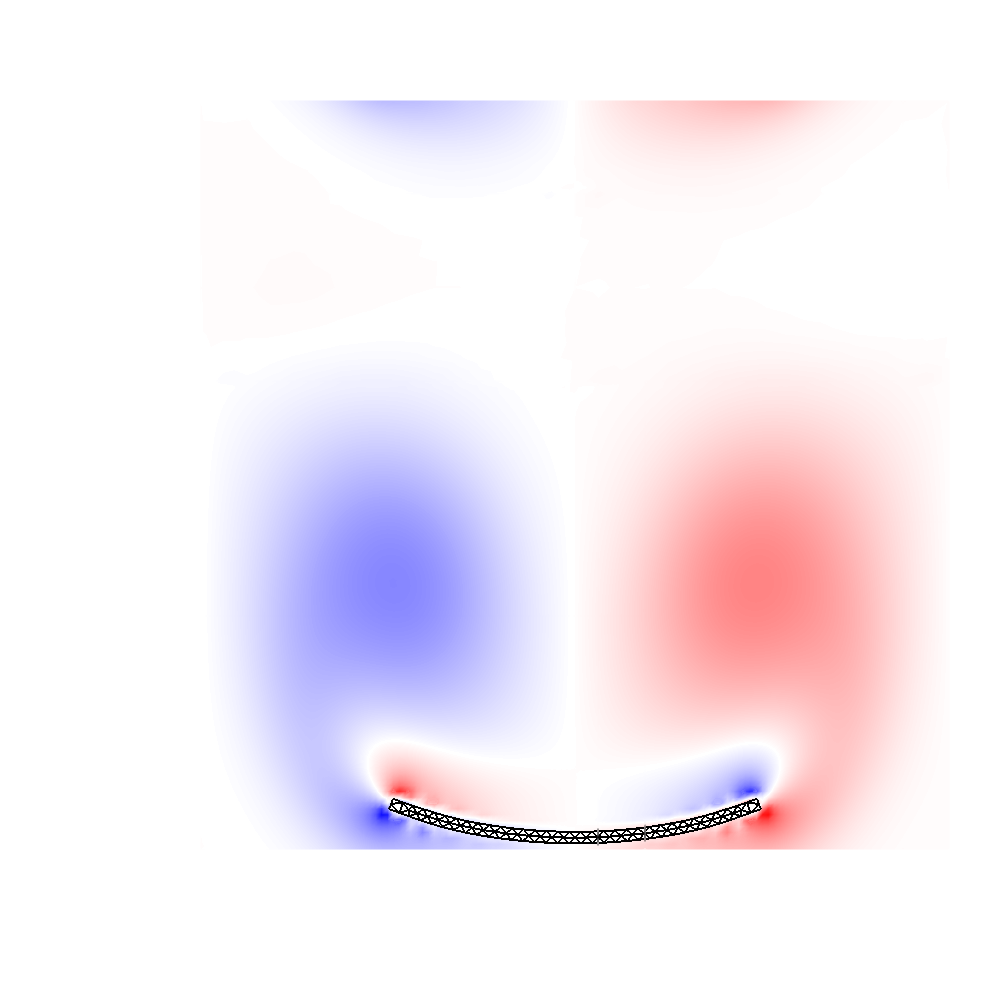
\includegraphics[width=\textwidth]{ch17-full-t4.png}\\ \scriptsize $t = 4$: still sinking, ends lagging
\end{columns}
\footnotesize
\begin{itemize}
  \item Vorticity $\pm 5$ (red positive, blue negative) on the fluid grid; the plate's mesh displaced by \code{dX}. The window is the whole $2\times2$ periodic box's centre $[-1,1]^2$.
  \item A plate pushed broadside sheds a vortex pair from its ends; the pair follows it down. After the release at $t = 3$ the fluid around the plate is still moving down and carries the plate with it: $y = -0.729$ at $t = 3.5$ and $-0.936$ at $t = 4$, with the ends behind the middle ($-0.877$). Nothing stops it but viscosity; in a longer run it would leave the box through the periodic bottom and reappear at the top.
\end{itemize}
\sourcecredit{IBFE/01, \code{MOTION = "FULL"}, IBAMR 0.19.0; \code{wsl/final/visit\_ch17.sh}.}
\end{frame}

% 31
\begin{frame}{HALF and ROTATE}
\label{fr:half}
\label{fr:rotate}
\begin{columns}[T]
\column{0.2\textwidth}\centering 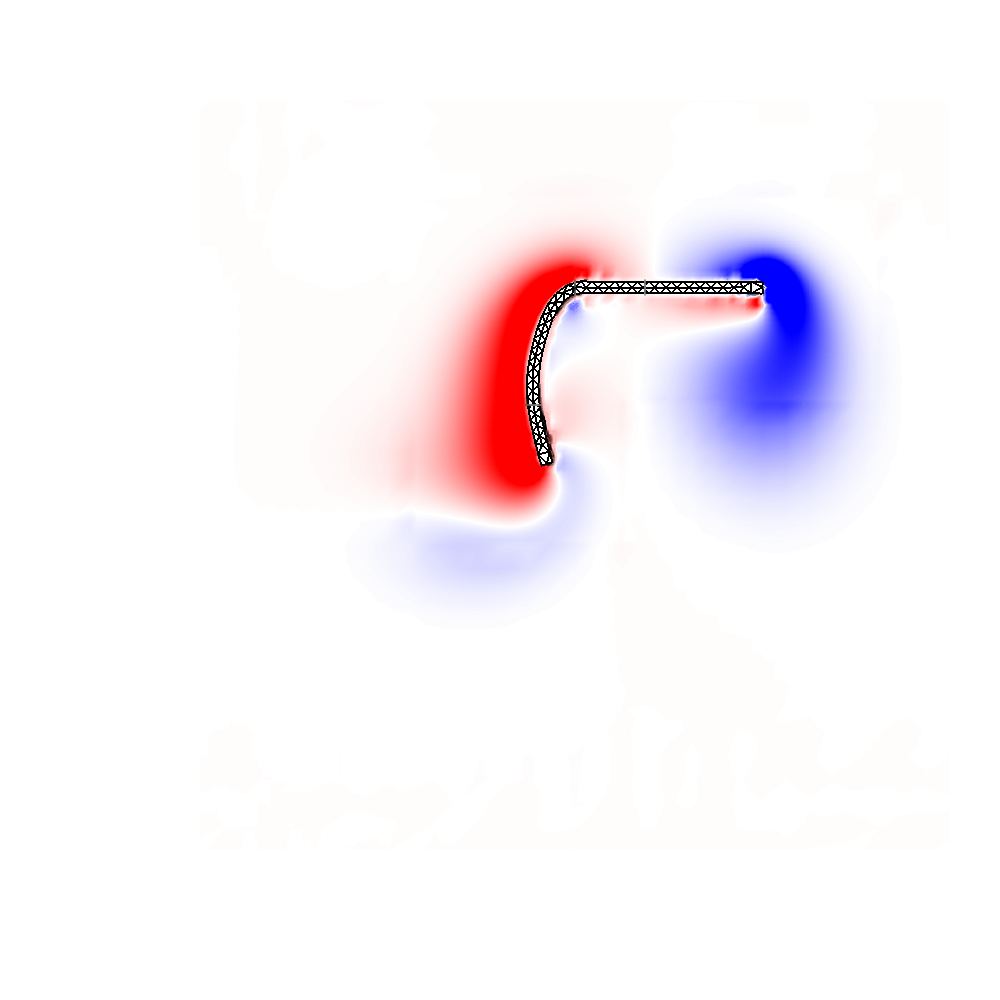
\includegraphics[width=\textwidth]{ch17-half-t1.png}\\ \scriptsize HALF, $t = 1$
\column{0.2\textwidth}\centering 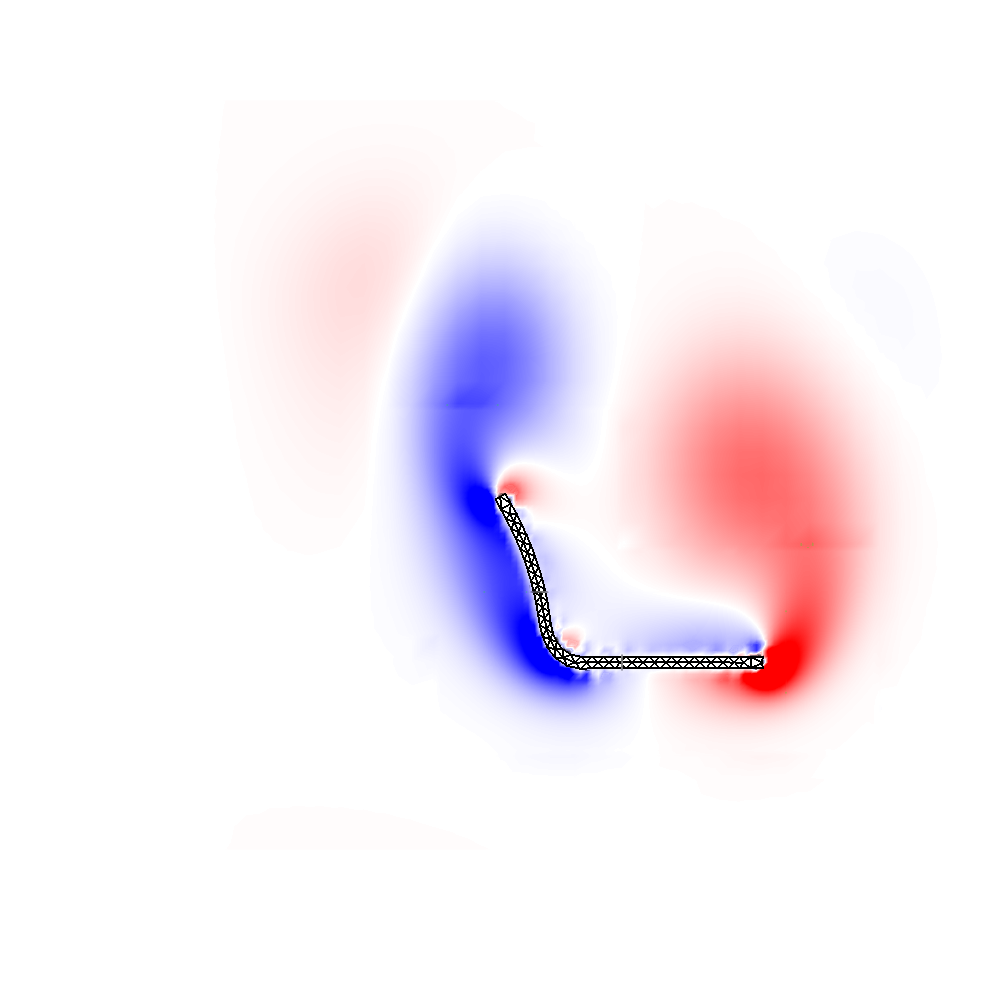
\includegraphics[width=\textwidth]{ch17-half-t3.png}\\ \scriptsize HALF, $t = 3$
\column{0.2\textwidth}\centering 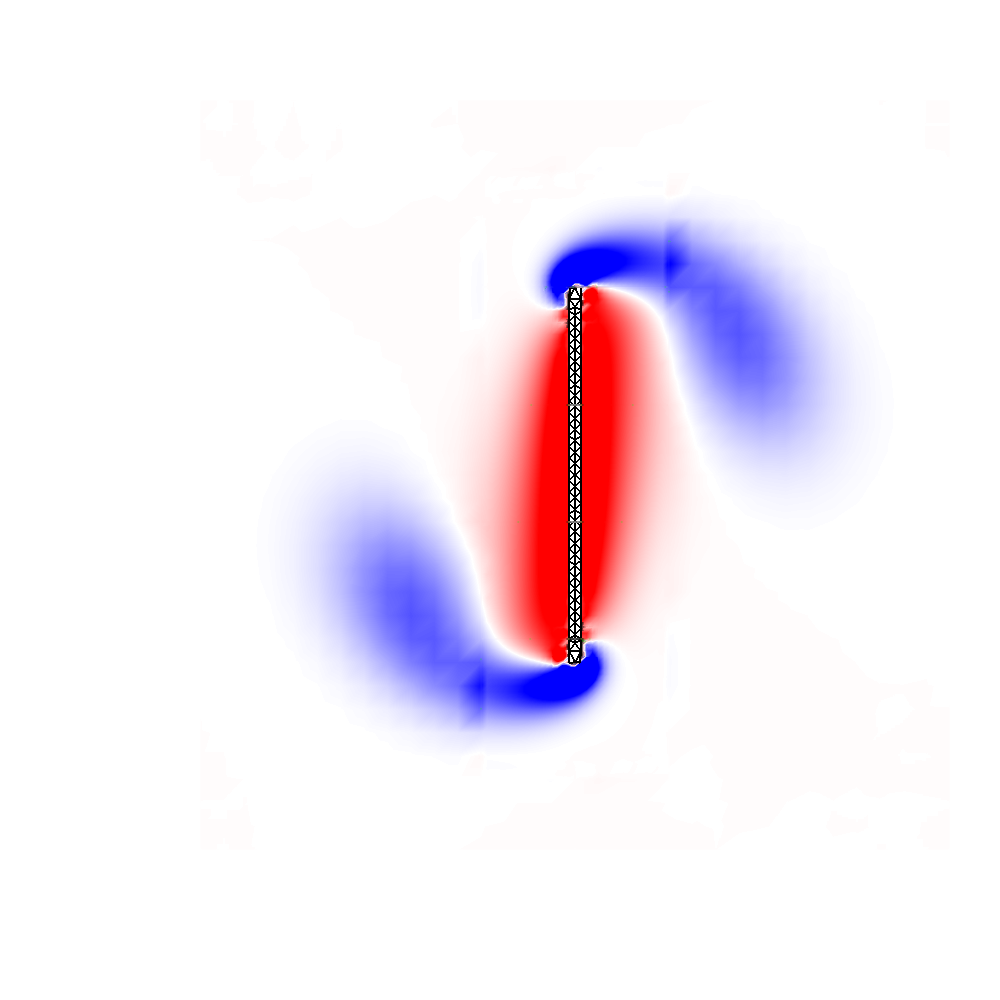
\includegraphics[width=\textwidth]{ch17-rotate-t1.png}\\ \scriptsize ROTATE, $t = 1$
\column{0.2\textwidth}\centering 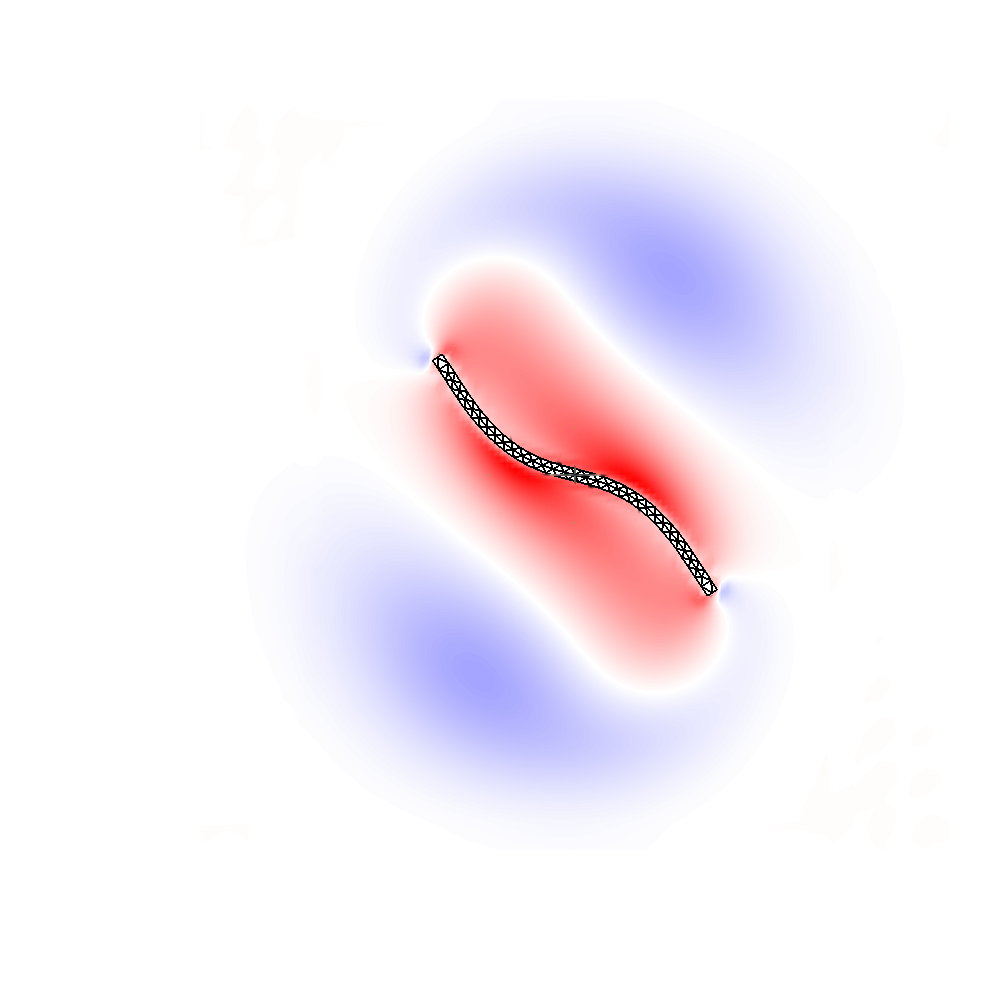
\includegraphics[width=\textwidth]{ch17-rotate-t2.png}\\ \scriptsize ROTATE, $t = 2$
\column{0.2\textwidth}\centering 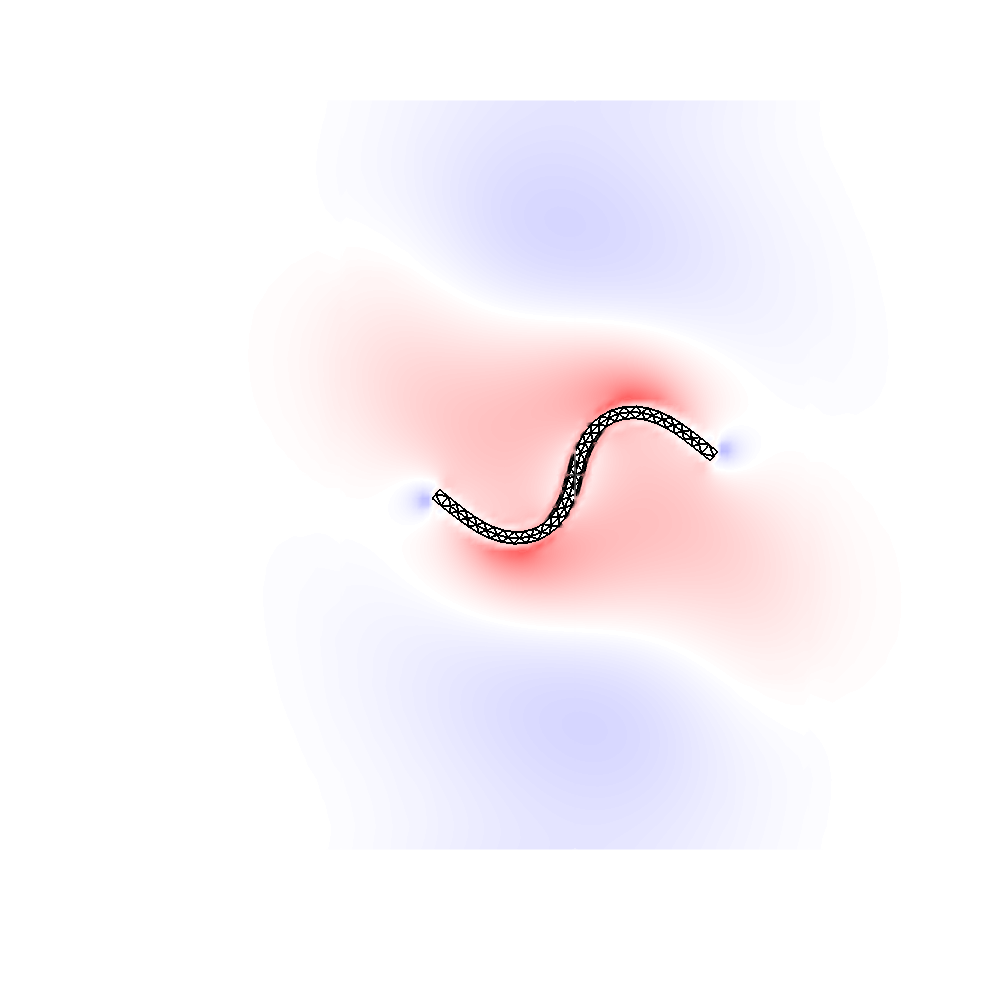
\includegraphics[width=\textwidth]{ch17-rotate-t4.png}\\ \scriptsize ROTATE, $t = 4$
\end{columns}
\footnotesize
\begin{itemize}
  \item \al{HALF}: the right tip follows the target exactly ($y = +0.500$ at $t = 1$, $-0.500$ at $t = 3$); the free left half lags, so the plate tilts by about $+39^\circ$ at $t = 1$ and about $-30^\circ$ from $t = 2$ on, and bends at the join between tethered and free material. The material law alone carries the left half.
  \item \al{ROTATE}: a quarter turn by $t = 1$, as prescribed, with the centre at the origin; released, the swirl the turn made keeps turning the plate, to about $140^\circ$ at $t = 2$ and $188^\circ$ at $t = 4$, while it bends in the flow it created.
\end{itemize}
\sourcecredit{IBFE/01, \code{MOTION = "HALF"} and \code{"ROTATE"}, IBAMR 0.19.0.}
\end{frame}

% 32
\begin{frame}{What was measured}
\label{fr:numbers}
\footnotesize
From \code{output.ex2} (the centre is the mean of the $101$ nodes; the tips are the nodes that start at $x = \pm 0.5$ on the centre line); IBAMR 0.16.0 and 0.19.0 agree:

\begin{columns}[T]
\column{0.42\textwidth}
\begin{tabular}{@{}lll@{}}
\toprule
FULL, time & centre $y$ & \\
\midrule
$0$ & $0.000$ & \\
$1.0$ & $+0.500$ & top \\
$2.0$ & $0.000$ & \\
$3.0$ & $-0.500$ & released \\
$3.5$ & $-0.729$ & carried by the fluid \\
$4.0$ & $-0.936$ & ends at $-0.877$ \\
\bottomrule
\end{tabular}
\column{0.54\textwidth}
\begin{tabular}{@{}L{0.30\textwidth}L{0.62\textwidth}@{}}
\toprule
run & result \\
\midrule
HALF & right tip $y = +0.500$ at $t = 1$, $-0.500$ at $t = 3$; tilt $+39^\circ$ ($t = 1$), $-30^\circ$ ($t \ge 2$) \\
ROTATE & $90^\circ$ at $t = 1$; $140^\circ$ at $t = 2$; $188^\circ$ at $t = 4$; centre at the origin throughout \\
\bottomrule
\end{tabular}
\end{columns}

\medskip
The 2014 and 2020 decks showed two renders each and no numbers; these are the acceptance test for the example: if your run gives these, your IBFE install works.
\end{frame}

% 32b
\begin{frame}{What was measured (2): a softer tether, a softer and a stiffer plate}
\label{fr:numbers2}
\footnotesize
\begin{tabular}{@{}L{0.30\textwidth}L{0.62\textwidth}@{}}
\toprule
change & result \\
\midrule
\code{KAPPA\_S = 1e4} & the plate trails its target ($y = 0.241$ instead of $0.250$ at $t = 0.5$) and overshoots when it turns ($0.507$ at $t = 1$) \\
\code{SHEAR\_MODULUS = 100}, HALF & fine; tilts less, about $32^\circ$ at $t = 1$ \\
\code{SHEAR\_MODULUS = 1}, HALF & the free half crumples (tip from $x = -0.5$ to $-0.15$ by $t = 1.5$), the flow it stirs up is fast, and the run stops near $t = 1.6$ with \code{Time step size change encountered}; halving \code{DT} delays the stop to $t \approx 2.05$ (chapter 16) \\
\bottomrule
\end{tabular}

\medskip
These are the ``Things to try'' of the example's README, run; chapter 8a's rule applies here too: change one parameter, predict, run, compare.
\end{frame}

% 33
\begin{frame}[fragile]{How the \code{.mat} mesh was made: the PDE Toolbox recipe}
\label{fr:pdetool}
\scriptsize
From the 2016 README (Julian Wag; the 2014 generic README promised this and never gave it). In MATLAB:
\begin{lstlisting}[style=matlab]
pdepoly([.5 .5 -.5 -.5], [.0156 -.0156 -.0156 .0156], 'g');   % the plate's outline, corners in order
\end{lstlisting}
This opens the PDE Modeler with the rectangle. \textbf{Mesh $\to$ Parameters}: maximum edge size two to four times the fine grid spacing ($0.0312$ was used); \textbf{Mesh $\to$ Initialize Mesh}; \textbf{Mesh $\to$ Export Mesh} with the default names \code{p}, \code{e}, \code{t}. Then write the file libMesh reads:
\begin{lstlisting}[style=matlab]
fid = fopen('IBFE_Mesh2D_128.mat', 'w');
fprintf(fid, '%d %d ', length(p), length(t));     % number of nodes, number of triangles
fprintf(fid, '%f %f ', p);                        % x y of each node
fprintf(fid, '%d %d %d %d ', t);                  % three node numbers and the subdomain of each triangle
fclose(fid);
\end{lstlisting}
\begin{itemize}
  \item \code{p} is $2\times N$ (coordinates), \code{t} is $4\times M$ (three nodes and a subdomain number); \code{fprintf} writes them column by column, which is the order of slide \ref{fr:matfile}.
  \item The README printed \code{fopen(IBFE\_Mesh2D\_128.mat'} with a curly quote and a missing one, which MATLAB rejects; the line above is the corrected one.
  \item The \code{.mat} name is libMesh's convention for this text format; do not \code{save} a MATLAB binary file under it.
  \item Without MATLAB: make the same plate with gmsh (chapter 18: a rectangle, \code{Mesh.CharacteristicLengthMax = 0.03}, export MSH 2.2 ASCII) and set \code{MESH\_FILENAME = "plate.msh"}; or with Triangle from a \code{.poly} file (next slide).
\end{itemize}
\end{frame}

% 34
\begin{frame}[fragile]{The \code{.poly} file that describes a different plate}
\label{fr:poly}
\footnotesize
Every course copy of this example shipped \code{Beam\_IBFE\_Mesh2D.m}. It does not write the \code{.mat} mesh; it writes a Triangle input file, \code{IBFE\_Mesh2D\_128.poly}, for a rectangle $1.0 \times 0.25$:
\begin{lstlisting}[style=matlabtiny]
L = 1.0; W = 0.25;                 % the beam's length and width
...
fid = fopen('IBFE_Mesh2D_128.poly','w');
fprintf(fid,'%d 2 0 0\n', Npts);   % nodes, dimension 2, no attributes, no boundary markers
...                                % the node lines, then the segment lines
\end{lstlisting}
\begin{itemize}
  \item The plate the example runs is $1.0 \times 0.0312$, eight times thinner, with $101$ nodes; the \code{.poly} rectangle, meshed with Triangle (\code{triangle -pq IBFE\_Mesh2D\_128.poly} gives \code{.node} and \code{.ele} files that libMesh reads, slide \ref{fr:formats}), is a different structure with different dynamics.
  \item The crosswalk found the mismatch when the example was ported; the script and its output are kept in \code{extras/} with a note, because a \code{.poly} file is one honest way to make a triangle mesh (chapter 18), and because readers of the old folders will meet it.
  \item \code{extras/beam\_ibfe\_mesh2d.py} writes an identical \code{.poly} without MATLAB.
\end{itemize}
\begin{punchbox}
\footnotesize When an example ships a generator script, check that the file it writes is the file the program reads: the name, the size and the number of nodes. Here two of the three differ.
\end{punchbox}
\end{frame}

% 35
\begin{frame}{What can go wrong}
\label{fr:wrong}
\footnotesize
\begin{tabular}{@{}L{0.36\textwidth}L{0.56\textwidth}@{}}
\toprule
symptom & cause and fix \\
\midrule
\code{Unknown MOTION = ...} & the key is misspelled; the valid words are printed with the error \\
\code{Illegal character token in input} at start-up & Windows line endings, or the stray \code{\textbackslash\textbackslash} at the end of the course input files; save as LF, delete the backslashes \\
\code{ERROR: Unrecognized file extension} and a list of formats & the mesh file's extension is not one libMesh knows (slide \ref{fr:formats}); rename, or convert with gmsh \\
no \code{output.ex2} & \code{viz\_dump\_interval = 0}, or the run never reached its first dump; the \code{"ExodusII"} word is not the switch (chapter 28) \\
the mesh does not move in VisIt & no Displace operator, or its variable is not \code{dX}; ``Apply operators to all plots'' was on and the operator landed on the fluid plot too \\
``mesh is 3D'' in VisIt, plate invisible against the fluid & an old IBAMR's three-coordinate 2D output: \code{\{dX\_0, dX\_1, 0\}} and the Project operator \\
\code{Time step size change encountered} & the plate is too soft for the flow it creates (\code{SHEAR\_MODULUS = 1}): a stiffer plate, a smaller \code{DT}, or accept it (chapter 16) \\
fluid leaks through the plate & too few quadrature points: raise \code{IB\_point\_density}; or the mesh is much coarser than the grid \\
a run restarted from \code{restart\_IB2d} starts \code{output.ex2} over & the writer was not told to append: \code{exodus\_io->append(from\_restart)} before the first write \\
\code{'AutoPtr' was not declared}, \code{libMeshEnums} & a course-era program against a current libMesh (slide \ref{fr:legacy}) \\
\bottomrule
\end{tabular}

\end{frame}

% 36
\begin{frame}[fragile]{What the older decks had that is now Part X}
\label{fr:legacy}
\scriptsize
\begin{tabular}{@{}L{0.46\textwidth}L{0.46\textwidth}@{}}
\toprule
2014--2020 & now \\
\midrule
Makefile: \code{LIBSNEW = \$(LIBS) -lnetcdf -lcurl},\newline\code{IBAMR\_SRC\_DIR = /nas02/apps/ibamr-3803/...}\newline or \code{.../ibamr-2016-11/...}, a \code{main-2d:} rule with \code{\$(LIBSNEW)} (the 2014 deck's slides 6--7; the 2020 deck's slide 6 with \code{/groups/lauram9/ib10/ibamr/...}) & \code{CMakeLists.txt} with \code{find\_package(IBAMR)}; libMesh, netCDF and curl come with the \code{IBAMR::IBAMR2d} target (chapter 3; the old flags in chapter X2) \\
\code{LibMeshInit init(argc, argv);}\newline\code{SAMRAI\_MPI::setCommunicator(PETSC\_COMM\_WORLD);}\newline\code{SAMRAIManager::startup();} & \code{IBTKInit ibtk\_init(argc, argv, MPI\_COMM\_WORLD);} \\
\code{Mesh mesh(NDIM)} (ibamr/3803) & \code{Mesh mesh(init.comm(), NDIM)} \\
\bottomrule
\end{tabular}

\end{frame}

% 36b
\begin{frame}[fragile]{What the older decks had that is now Part X (2)}
\label{fr:legacy2}
\scriptsize
\begin{tabular}{@{}L{0.46\textwidth}L{0.46\textwidth}@{}}
\toprule
2014--2020 & now \\
\midrule
\code{target\_force\_function(F, FF, X, s, elem,}\newline\code{const vector<NumericVector<double>*>\& system\_data,}\newline\code{time, ctx)}: seven arguments & the nine of slide \ref{fr:signature}: \code{var\_data} and \code{grad\_var\_data} in place of \code{system\_data} \\
\code{libMeshEnums::Order} & \code{libMesh::Order} \\
\code{AutoPtr<ExodusII\_IO> exodus\_io(new ExodusII\_IO(mesh))} & \code{std::unique\_ptr<ExodusII\_IO>} \\
\code{\#include <IBAMR\_config.h>}, \code{<IBTK\_config.h>} & removed \\
\code{s\_dump(1)=s(1)+s(0)*sin(2*3.14*0.5*time)} & an exact rotation with \code{PI} (slide \ref{fr:rotatecode}) \\
\bottomrule
\end{tabular}

\medskip
The old programs compile against the 0.16.0--0.19.0 headers only after all of these; chapter X3 lists the error messages each one produces (\code{'AutoPtr' was not declared}, \code{fatal error: IBAMR\_config.h}, the \code{IBFEMethod(...)} constructor mismatch of the multi-mesh programs).
\end{frame}

% 37
\begin{frame}{Exercises}
\label{fr:exercises}
\footnotesize
\begin{enumerate}
  \item Translate the plate to the left at $0.3$ for one second (the 2014 slide 10), then release it. Where is its centre at $t = 2$? Compare with FULL's drift after release.
  \item Add the sinusoidal body force of slide \ref{fr:sinus} (a new \code{MOTION = "SHAKE"} case, with the amplitude and frequency in the input) and run it for four periods, once on the ends as the 2016 code does and once on the middle half as the 2014 slide says. Which part of the plate moves most, and why is it not the forced part alone?
  \item Repeat FULL with \code{KAPPA\_S = 1e4} and \code{1e2}. At which stiffness does the plate stop following the target, and what does the vorticity look like then?
  \item Repeat HALF with \code{SHEAR\_MODULUS = 1} and watch the run stop. Read chapter 16's slide on \code{Time step size change encountered}, then find the largest \code{DT} that reaches $t = 4$.
  \item Make the same plate in gmsh (chapter 18), run FULL with \code{MESH\_FILENAME} set to it, and compare the centre positions of slide \ref{fr:numbers}. Then halve the element size and compare again.
  \item Put a pressure load of slide \ref{fr:surface} on the plate (no tether: \code{MOTION = "FULL"} with \code{KAPPA\_S = 0}) and explain what a uniform pressure on a closed boundary does to a nearly incompressible body.
\end{enumerate}
\end{frame}

% 38
\begin{frame}{Rules of thumb}
\label{fr:thumb}
\small
\begin{itemize}
  \item Four things: a mesh, a stress function, a force function, the registrations. Everything else is the chapter 5 program.
  \item Write prescribed motion as a target position in the reference configuration; release by setting the target to the current position.
  \item \code{s(0)} is $x$ and \code{s(1)} is $y$ in the reference configuration; \code{X} is the current position. IBAMR's headers call them \code{X} and \code{x}.
  \item One body force function per part, any number of stress functions; each stress function gets its own quadrature order.
  \item \code{viz\_writer = "VisIt","ExodusII"}: what the examples write; the plate file comes with the visualization dumps whether or not the second word is there (chapter 28).
  \item In VisIt the mesh is drawn where it started until you displace it by \code{dX = \{dX\_0, dX\_1\}}.
  \item \code{MFAC} and \code{ELEM\_TYPE} do nothing to a mesh read from a file; \code{IB\_point\_density} does.
  \item Check that a shipped generator writes the file the program reads.
\end{itemize}
\end{frame}

% 39
\begin{frame}{Summary}
\label{fr:summary}
\footnotesize
\begin{enumerate}
  \item IBFE replaces points, springs and beams by a finite element mesh with a material law. Forces come from a first Piola--Kirchhoff stress function and from body and surface force functions, all C++ callbacks with the nine- (or twelve-) argument signature, and are spread from quadrature points.
  \item Example IBFE/01 is the course's three tether examples in one program: a plate pulled up and down, half of it, or turned; \code{MOTION} picks one. It builds with the six-line CMake file and runs in under a minute; the numbers of slide \ref{fr:numbers} are its acceptance test.
  \item The input adds a handful of IBFE keys; \code{IB\_point\_density} and the quadrature orders matter for any mesh, \code{MFAC} and \code{ELEM\_TYPE} only for a mesh built in the program.
  \item The plate's output is one ExodusII file with the reference mesh and \code{dX}; VisIt needs the \code{dX} expression and the Displace operator to draw it where it is.
  \item Ten years of versions left a handful of slips: the \code{s(1)} comment, the sheared ``rotation'', $2\cdot 3.14$, the half-turn that was called a spin, the \code{.poly} generator for another plate, the curly quote in the README, the ``1.0 is better'' comments. All are corrected in the example and recorded here.
\end{enumerate}
\begin{homebox}
\footnotesize Chapter 18 makes meshes: gmsh, Triangle and TetGen, Coreform Cubit, libMesh's generators, and the element-size rules. Chapter 19 writes the stress functions properly.
\end{homebox}
\end{frame}

% 40
\begin{frame}{Recordings (listed, not incorporated)}
\label{fr:videos}
\small Shannon Jones's YouTube tutorial on visualizing IBFE boundaries in VisIt (\code{youtube.com/watch?v=Kj\_MACemSd0}; the IBFE Read Me warns that it has a mistake the slides correct), and the 2020 Zoom recordings of the IBFE lectures, are listed in the front matter's video list (chapter 0.1). Nothing in them is reproduced here.
\end{frame}

% 41
\begin{frame}{References and credits}
\label{fr:refs}
\scriptsize
\begin{itemize}
  \item B. E. Griffith and X. Luo, \emph{Hybrid finite difference/finite element immersed boundary method}, International Journal for Numerical Methods in Biomedical Engineering 33 (2017) e2888. \url{https://doi.org/10.1002/cnm.2888}; \url{https://arxiv.org/abs/1612.05916}.
  \item IBAMR 0.19.0: \code{include/ibamr/IBFEMethod.h}, \code{include/ibamr/FEMechanicsBase.h}, \code{src/IB/IBFEMethod.cpp} (\code{getFromInput}), \code{ibtk/include/ibtk/libmesh\_utilities.h}, \code{ibtk/include/ibtk/IBTKInit.h}; \url{https://github.com/IBAMR/IBAMR}. libMesh 1.7.8: \code{src/mesh/namebased\_io.C}, \code{matlab\_io.C}; \url{https://libmesh.github.io}.
  \item The example of this series: \code{examples/IBFE/01-tethered-plate} (\code{main.cpp}, \code{input2d}, \code{IBFE\_Mesh2D\_128.mat}, \code{CMakeLists.txt}, \code{job.slurm}, \code{README.md}, \code{extras/}); figures by \code{wsl/final/visit\_ch17.sh}.
  \item Sources: Alex Hoover, \emph{1-IBFE Tutorial: Getting Started} (UNC, 2014, edited 2017, 18 slides) and the examples' README files (Hoover 2014; Julian Wag 2016); \emph{1-IBFE Getting Starting and Visualizing a Mesh} (MATH 769, 2018, 27 slides; lab versions 2020--2024, 26 slides); \emph{IBFE Read Me} (2017). The course examples were developed with Alex Hoover, Julian Wag and Nick Battista (2014--2018) and revised at the University of Arizona (2022--2024).
\end{itemize}
\end{frame}

\end{document}
